\chapter{Experimental Results}

\section{Circuit Construction}

\subsection{Non-Inverting Amplifier}

\begin{figure}[h]
    \centering
    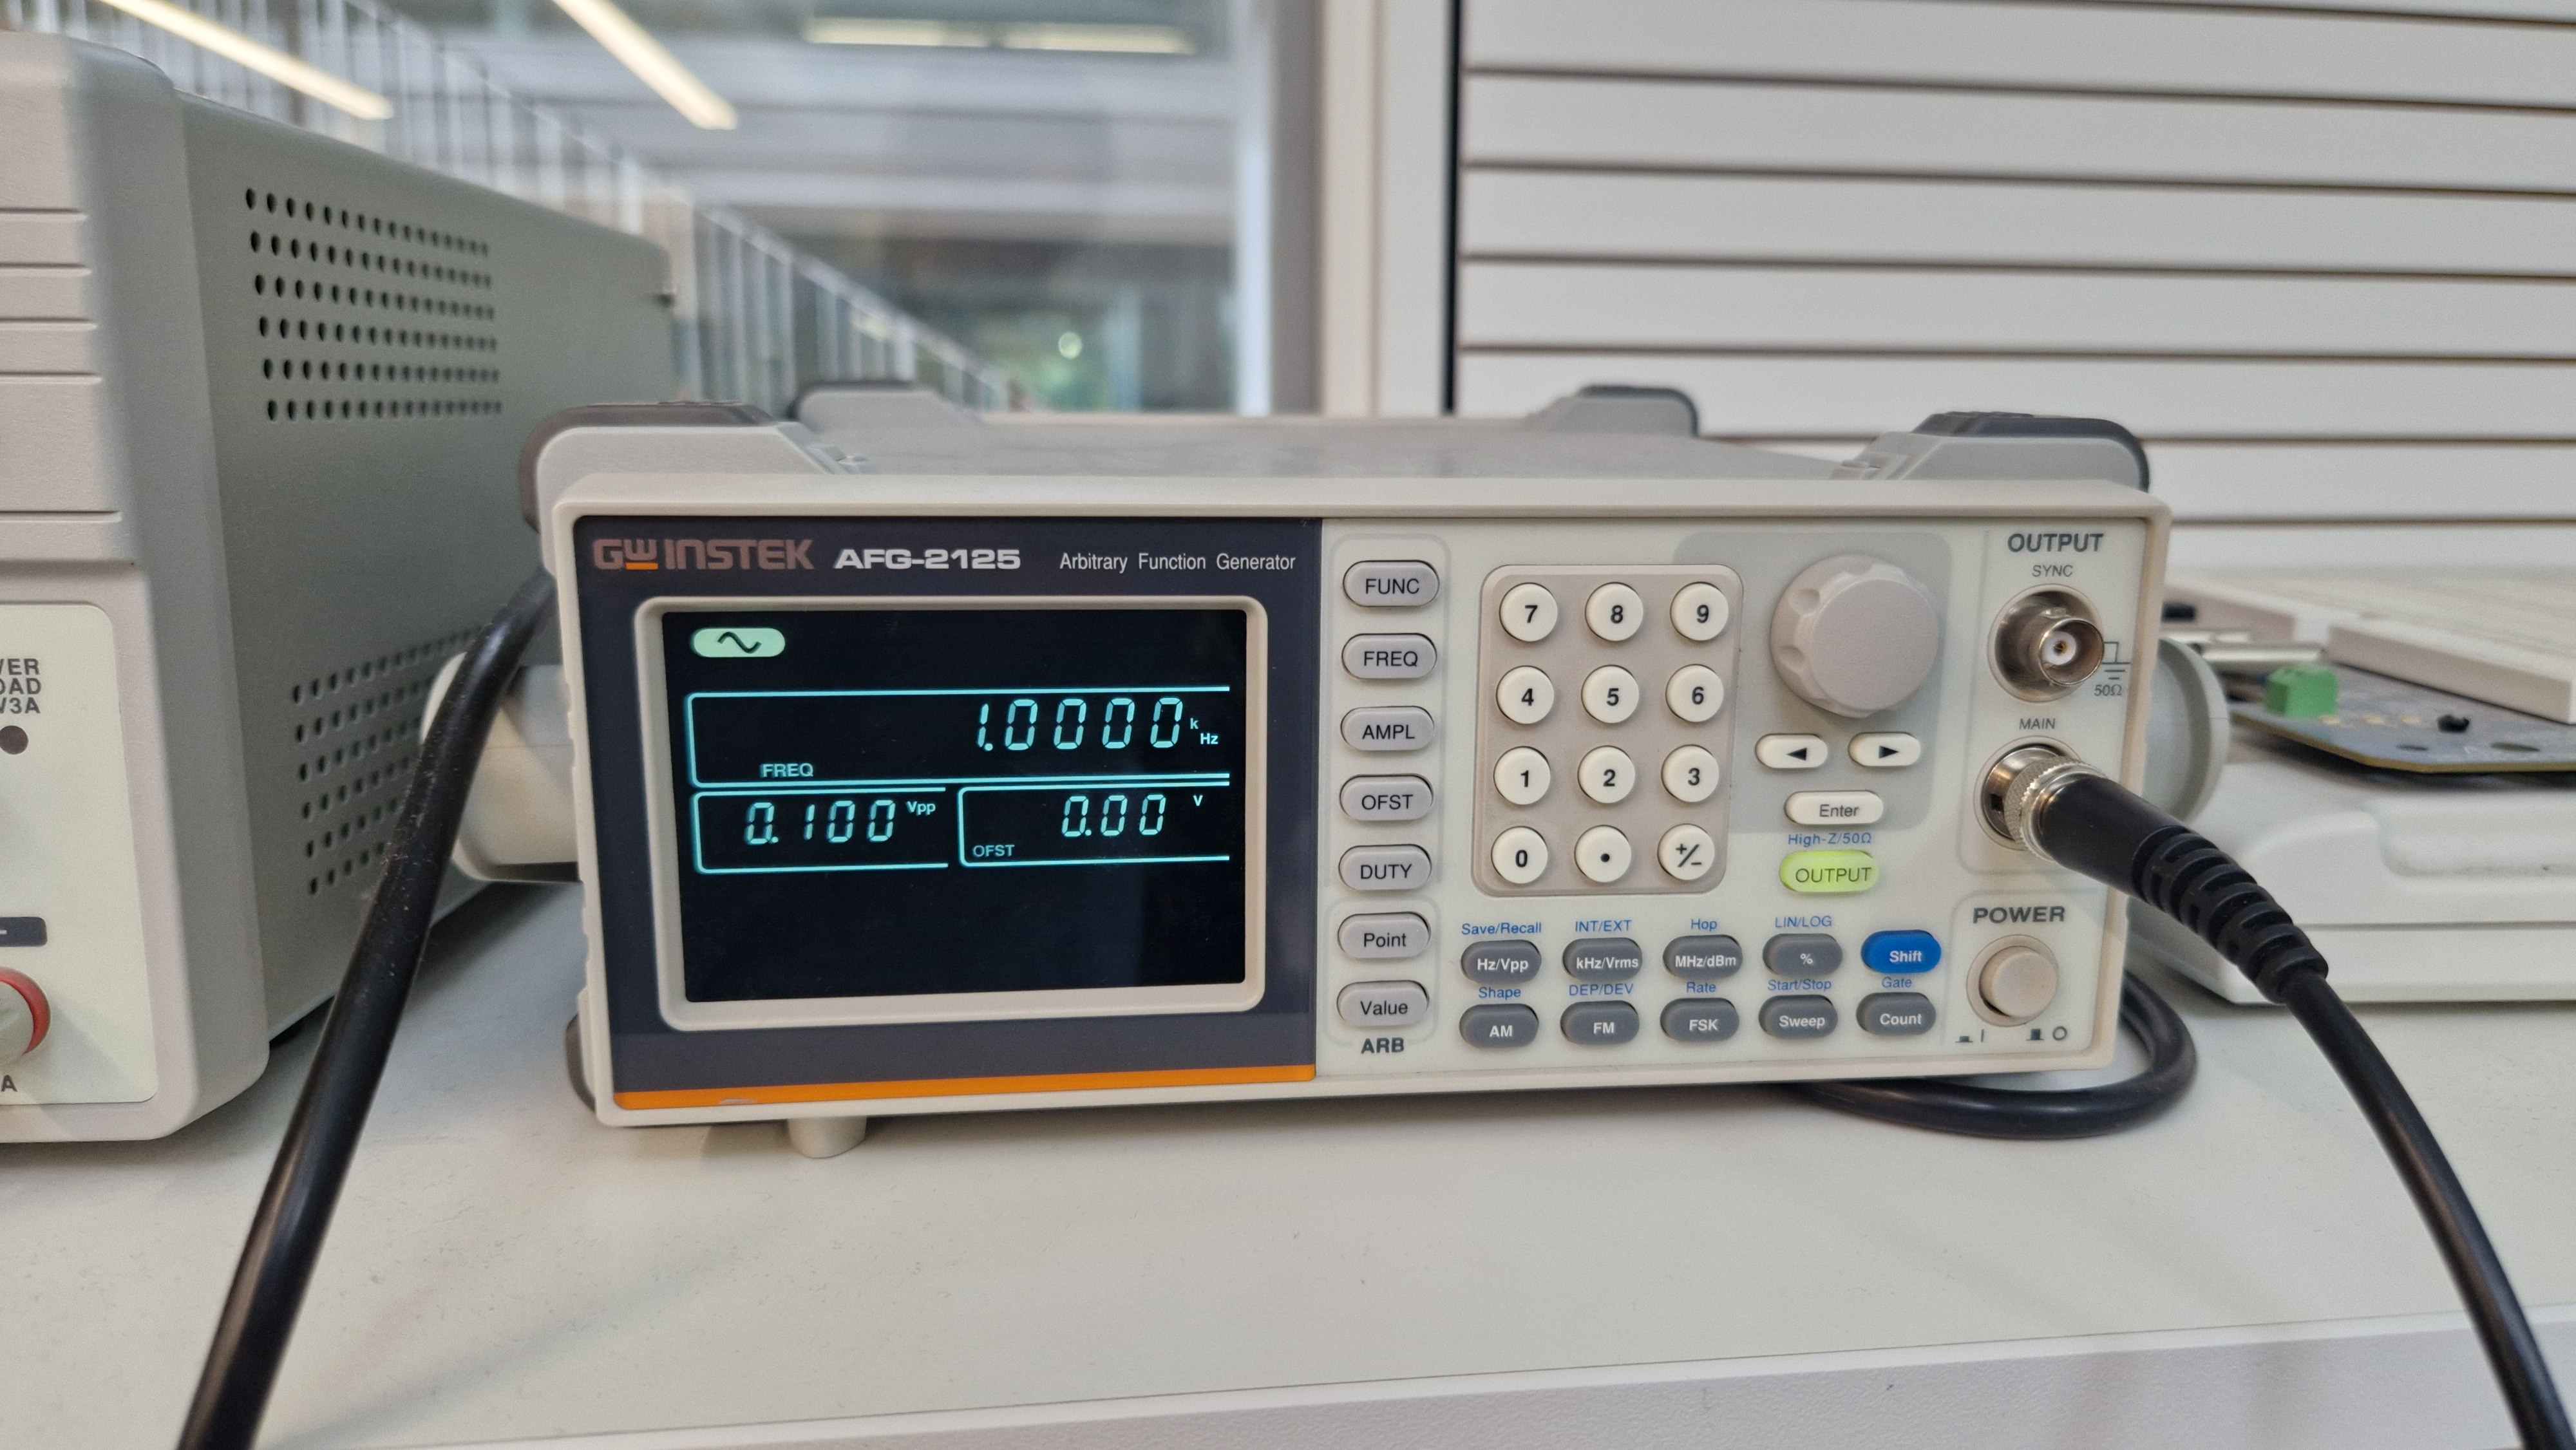
\includegraphics[width=0.6\textwidth]{assets/non-inverting-100m.jpg}
    \caption{Signal Generator @ 100mV}
    \label{fig:non-inverting-100m}
\end{figure}

\begin{figure}[h]
    \centering
    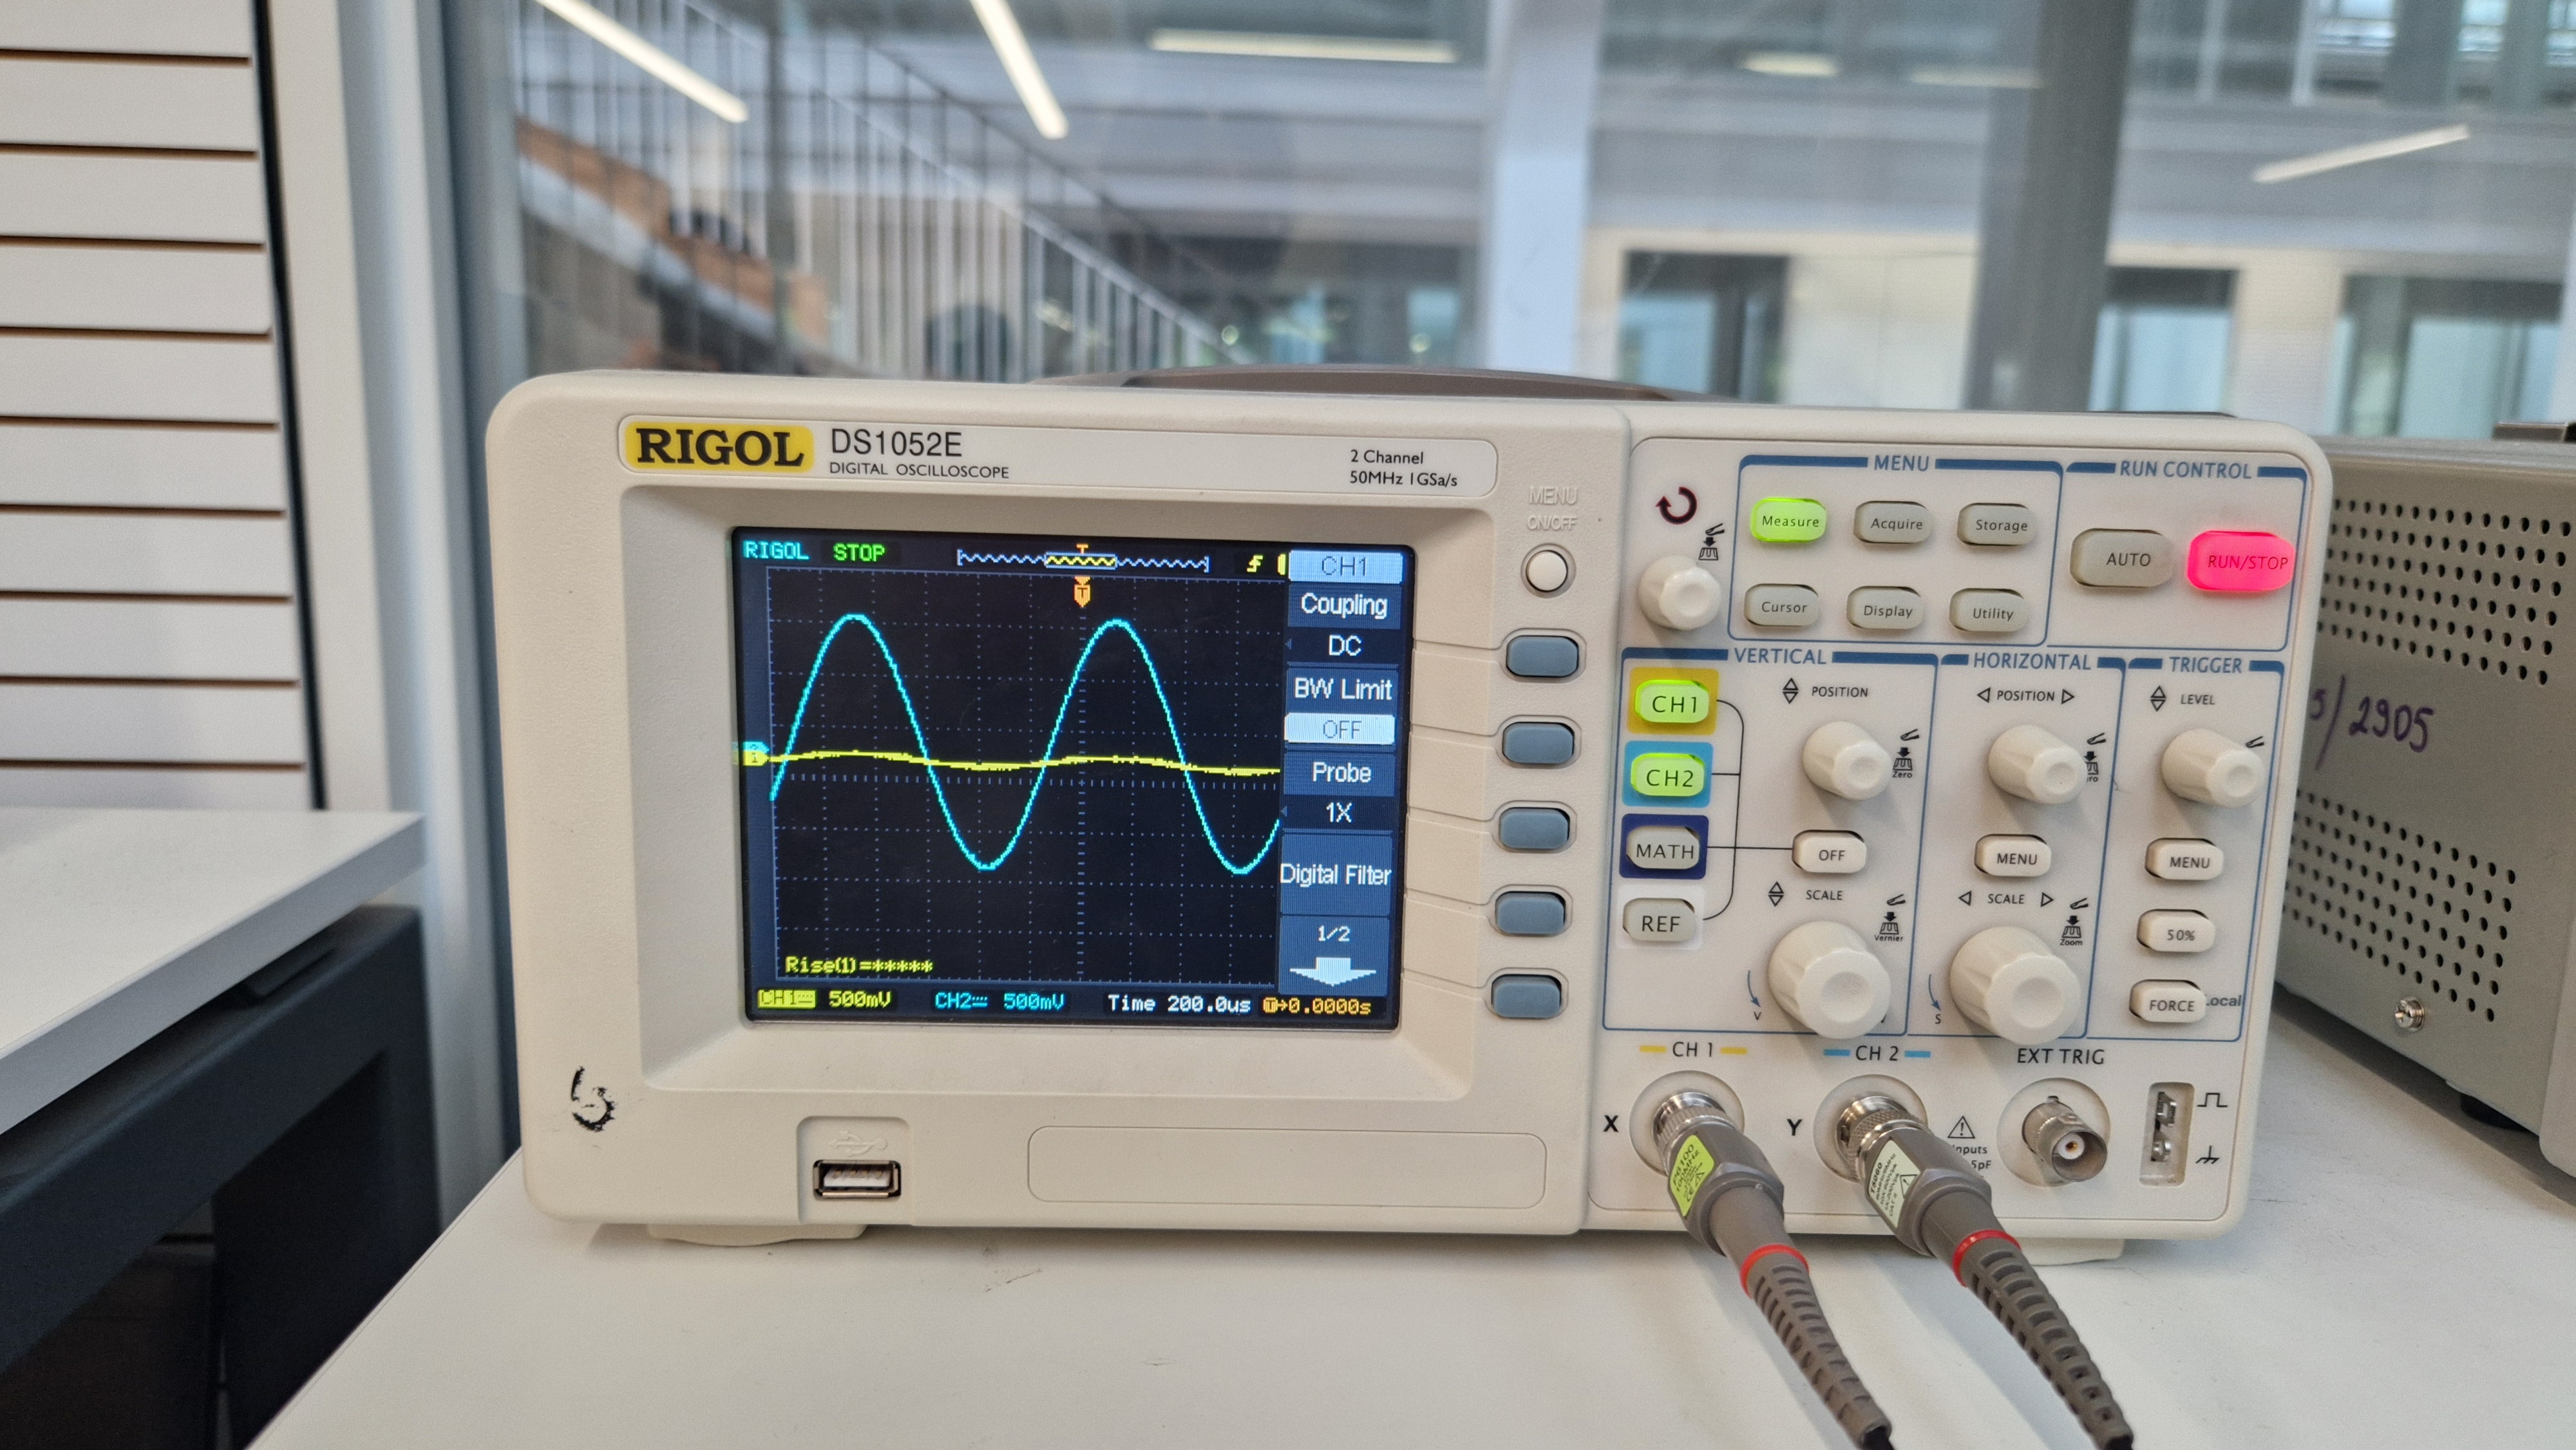
\includegraphics[width=0.6\textwidth]{assets/non-inverting-100m-output.jpg}
    \caption{Non-inverting @ 100mV}
    \label{fig:non-inverting-100m-output}
\end{figure}

Applying 100mV input to the non-inverting amplifier, the output is close to 2.3V as expected. The experiment result is shown in Figure \ref{fig:non-inverting-100m-output}. 

\newpage
\thispagestyle{plain}

\begin{figure}[h]
    \centering
    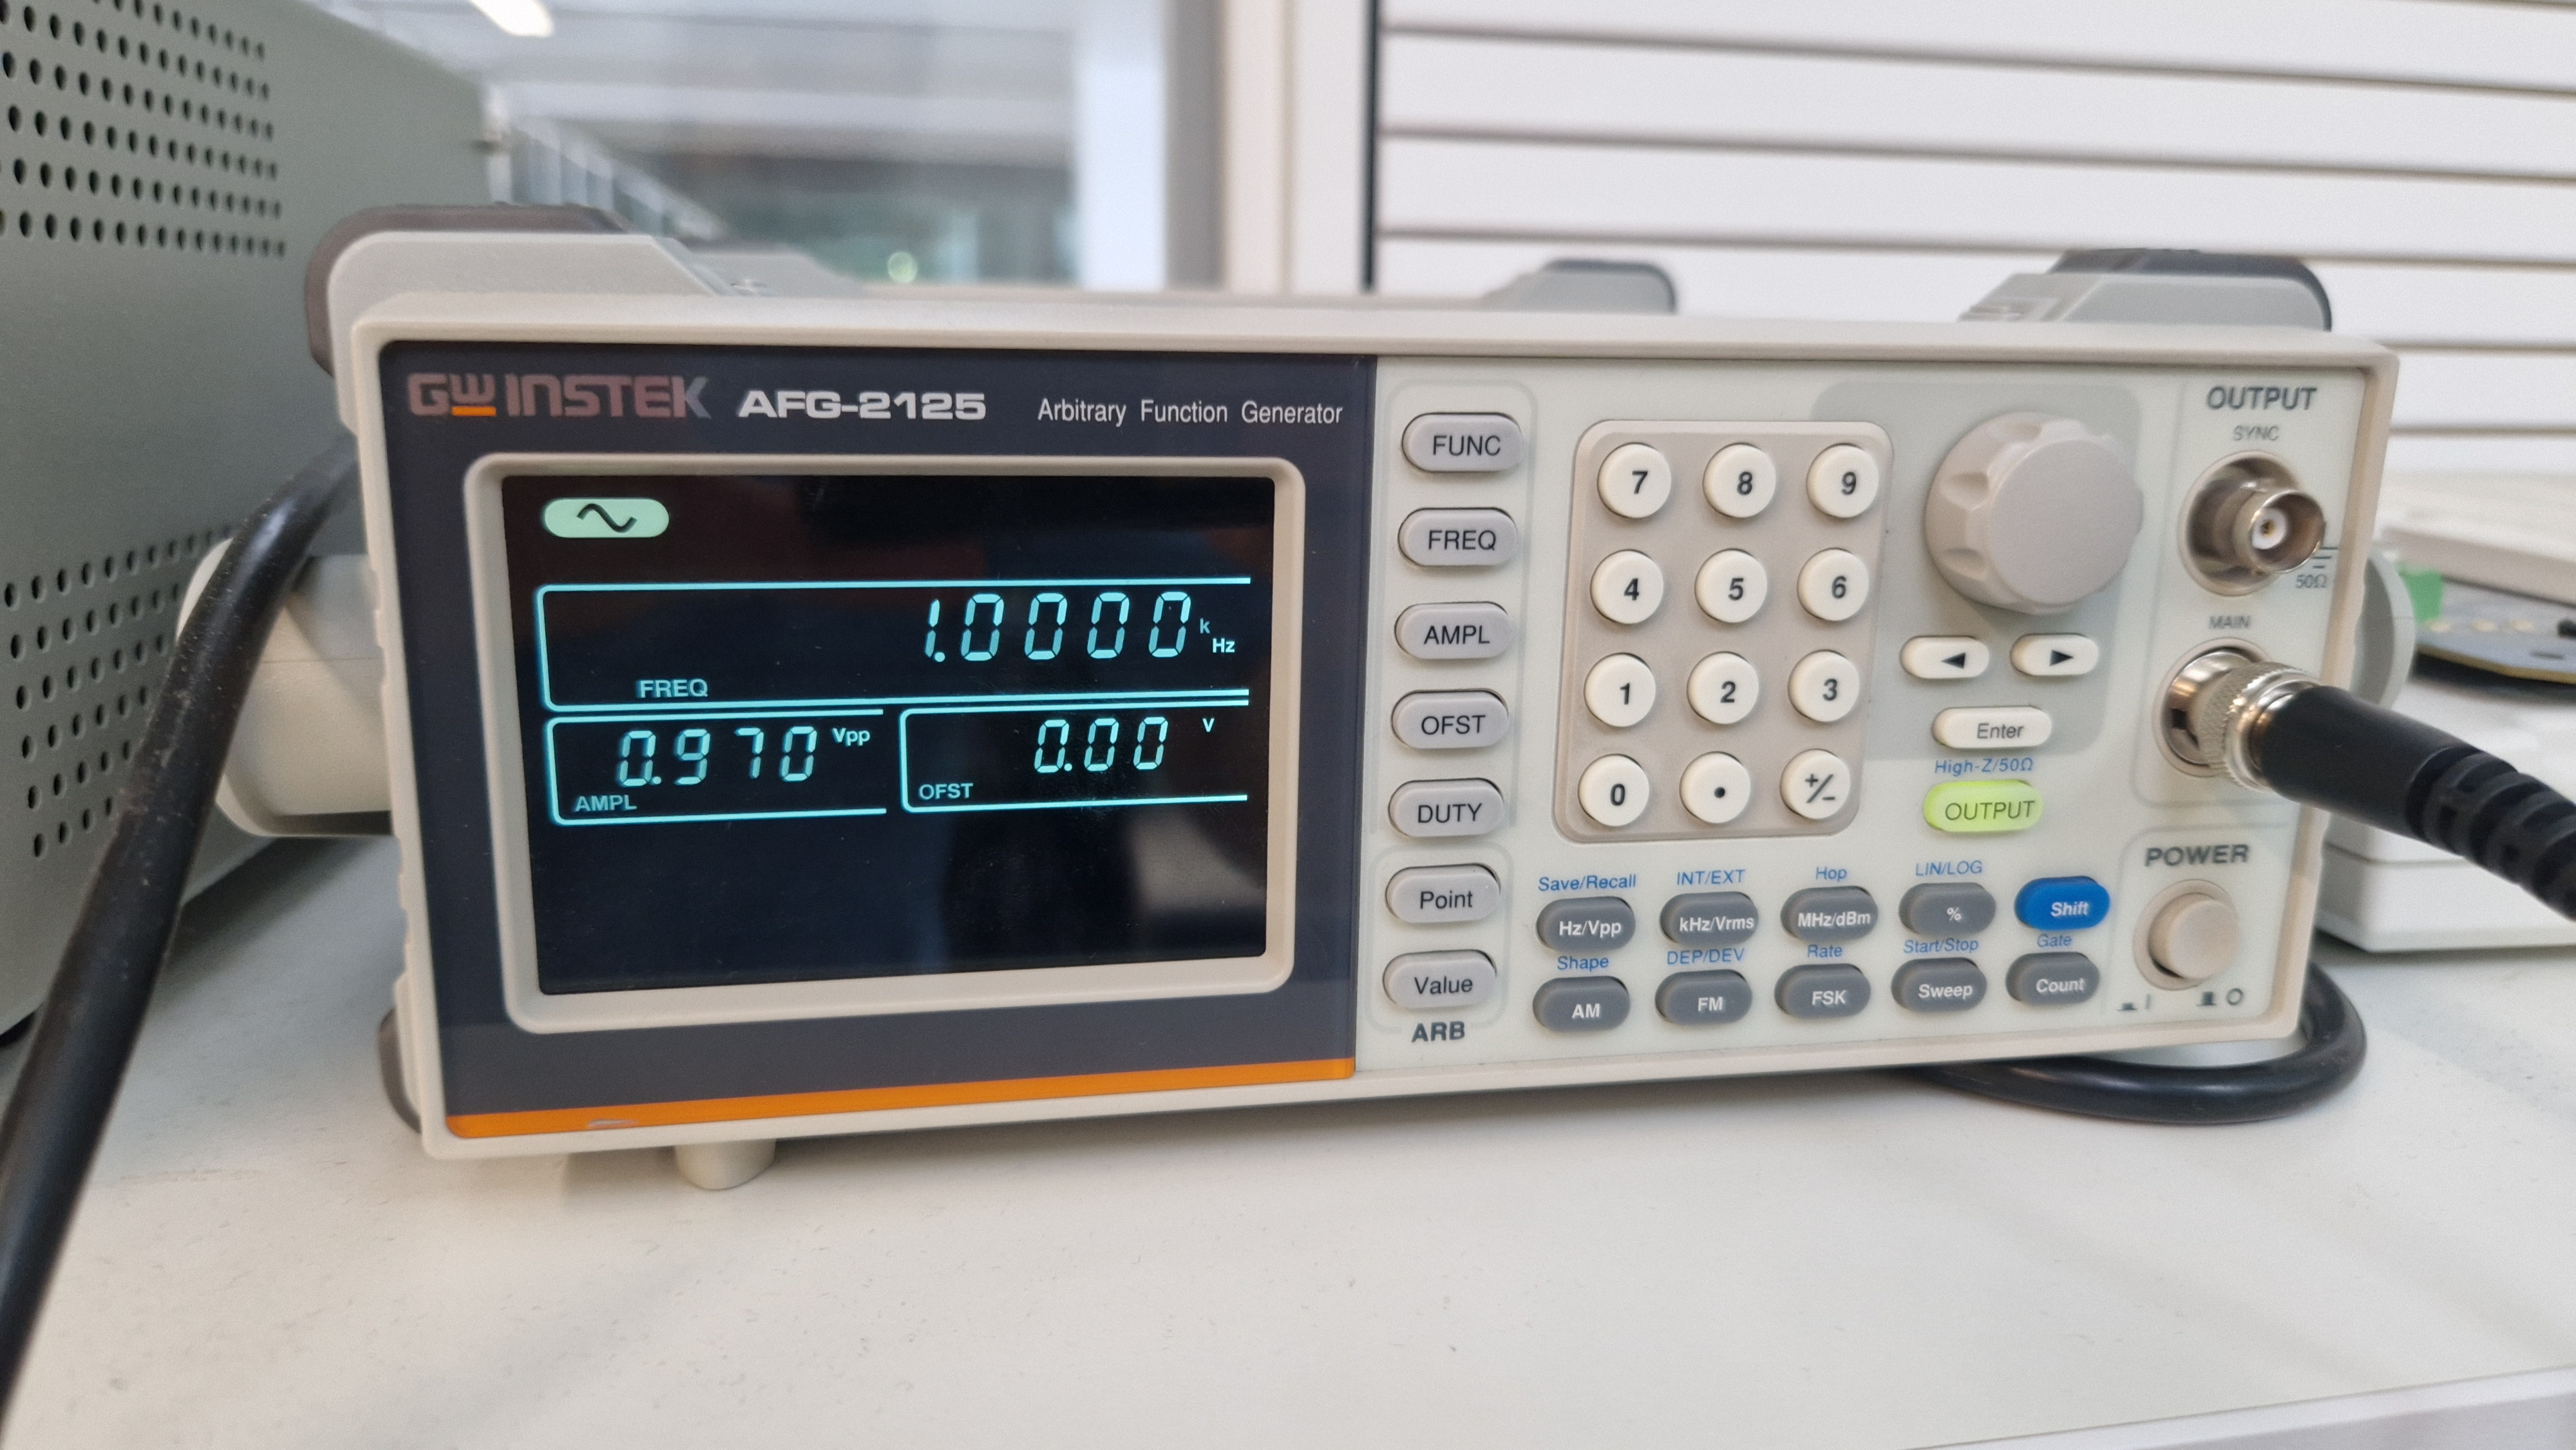
\includegraphics[width=0.6\textwidth]{assets/non-inverting-970m.jpg}
    \caption{Signal Generator @ 970mV}
    \label{fig:non-inverting-970m}
\end{figure}

\begin{figure}[h]
    \centering
    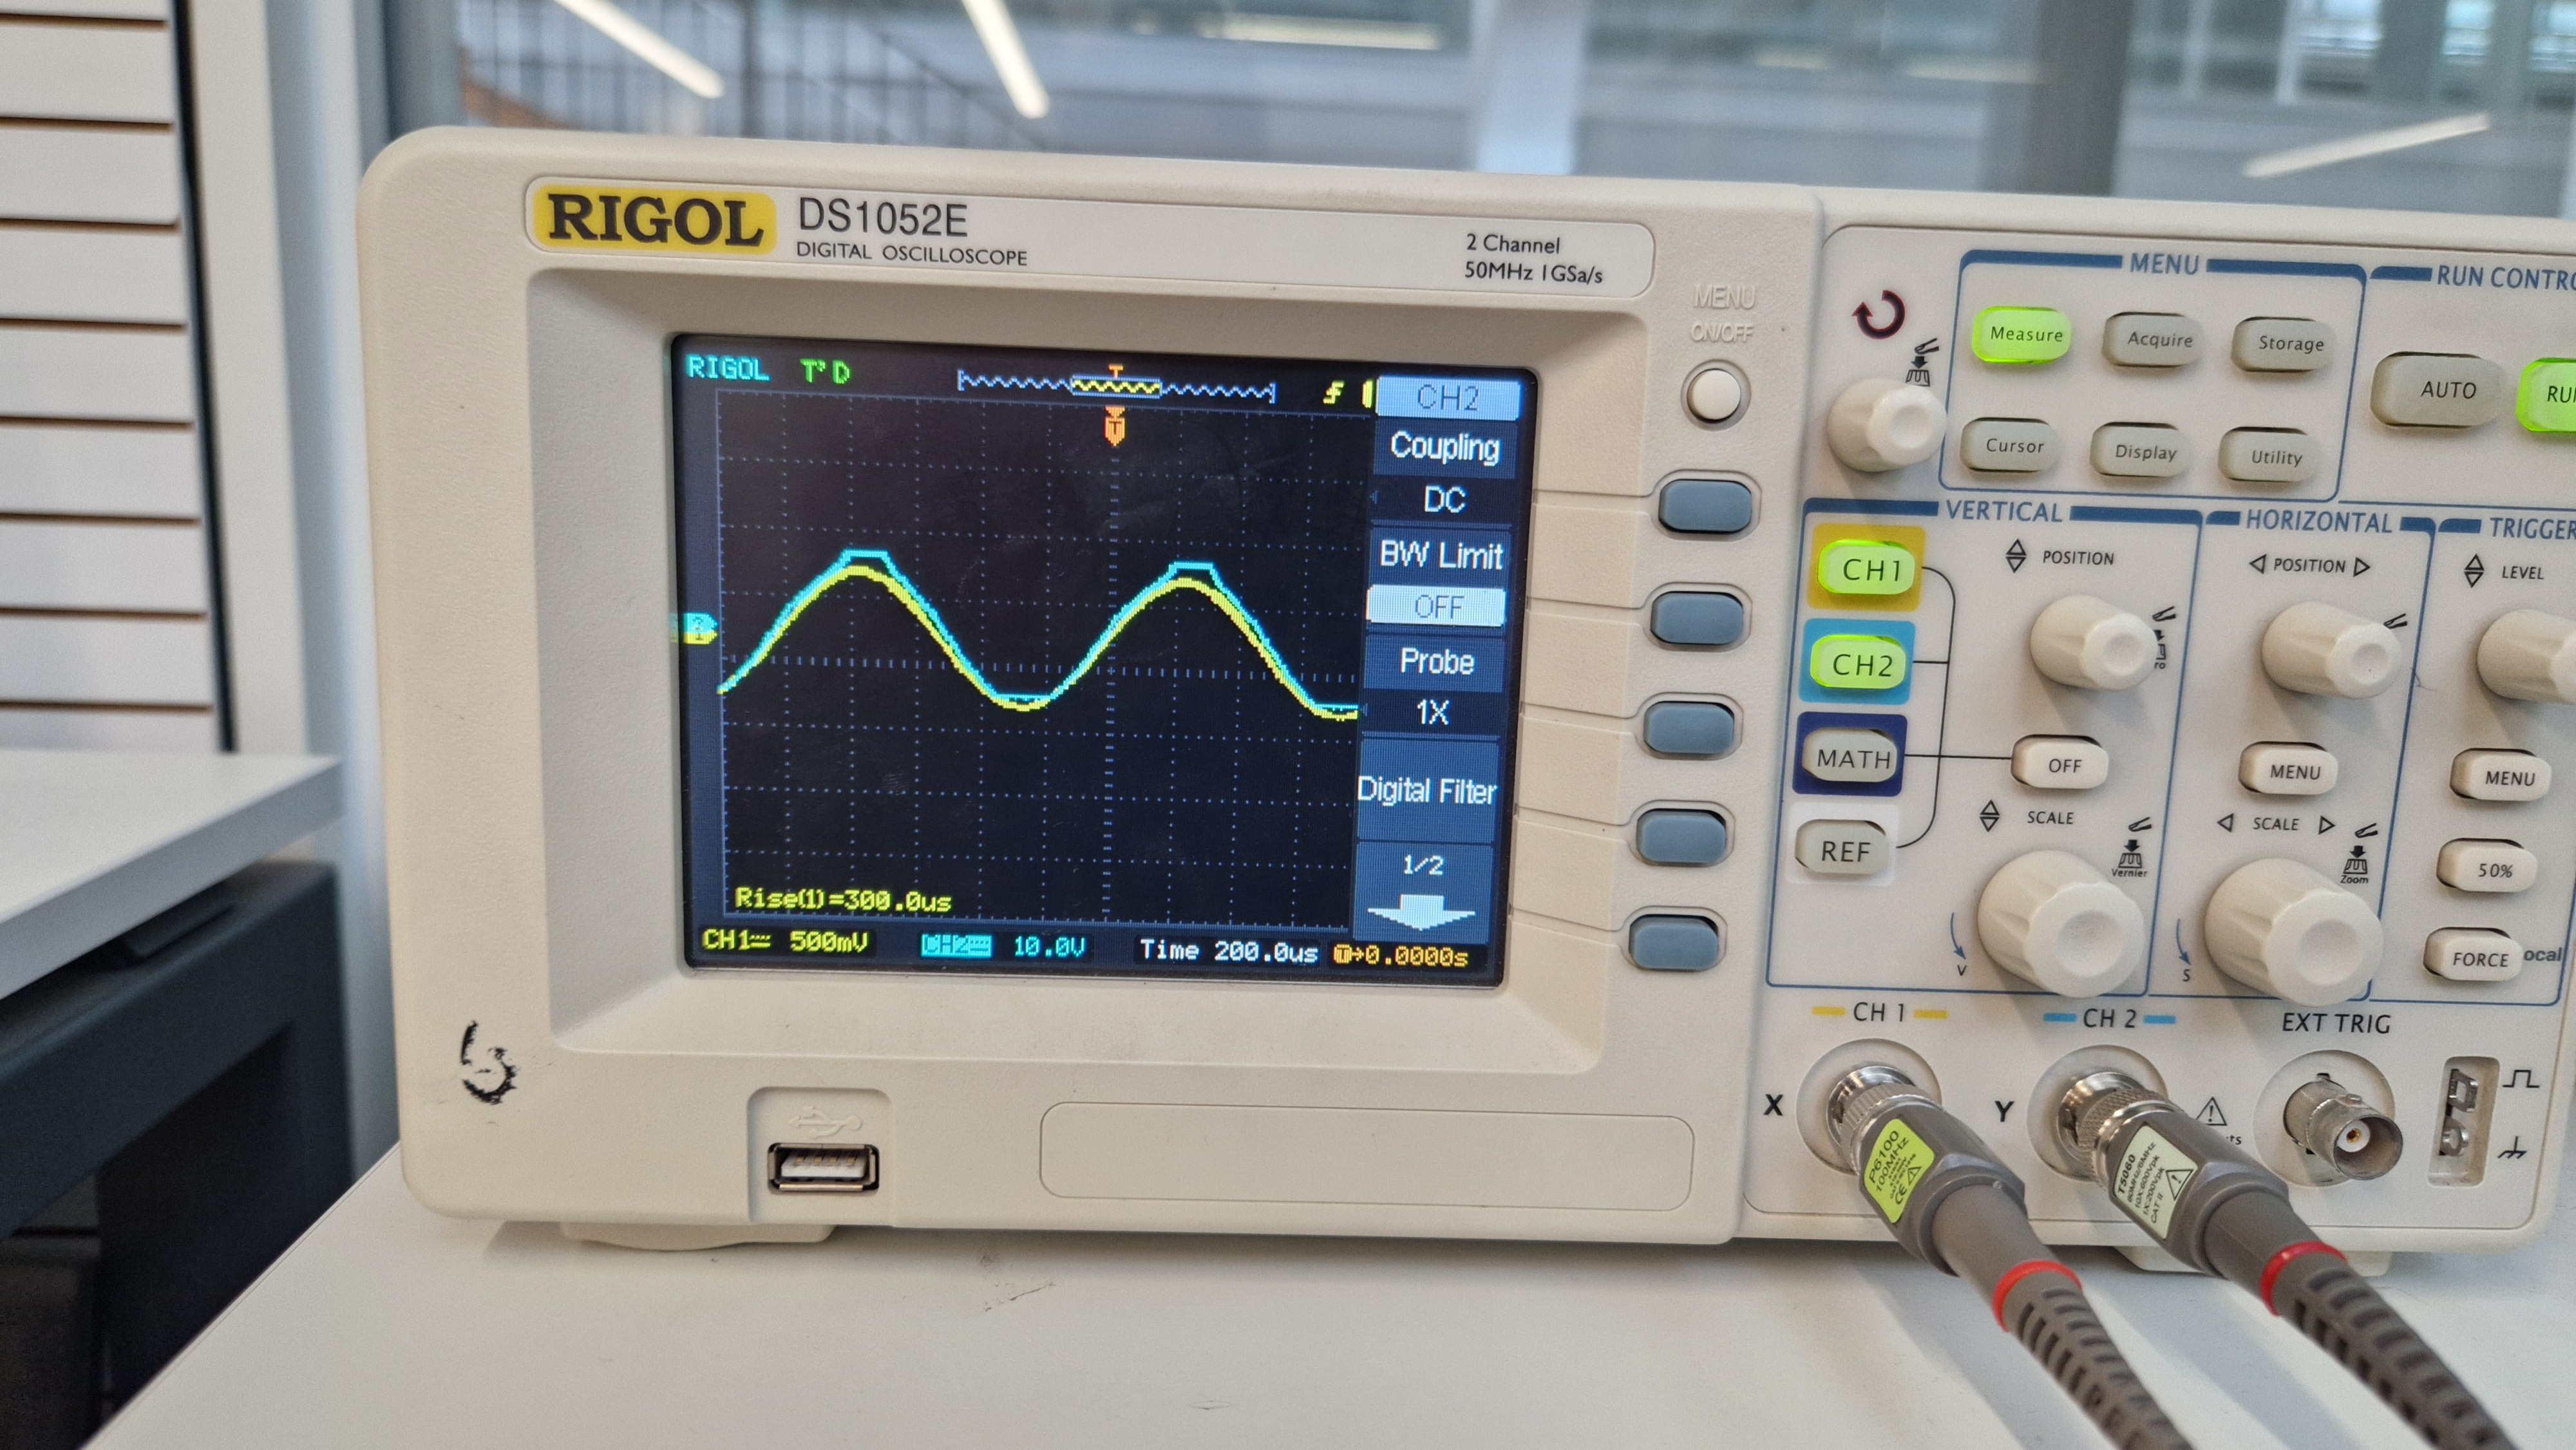
\includegraphics[width=0.6\textwidth]{assets/non-inverting-970m-output.jpg}
    \caption{Non-inverting @ 970mV}
    \label{fig:non-inverting-970m-output}
\end{figure}

Applying 970mV input to the non-inverting amplifier, the output should be 13.7V but it is limited to 12V due to the power supply as seen in Figure \ref{fig:non-inverting-970m-output}.

\newpage
\thispagestyle{plain}

\begin{figure}[h]
    \centering
    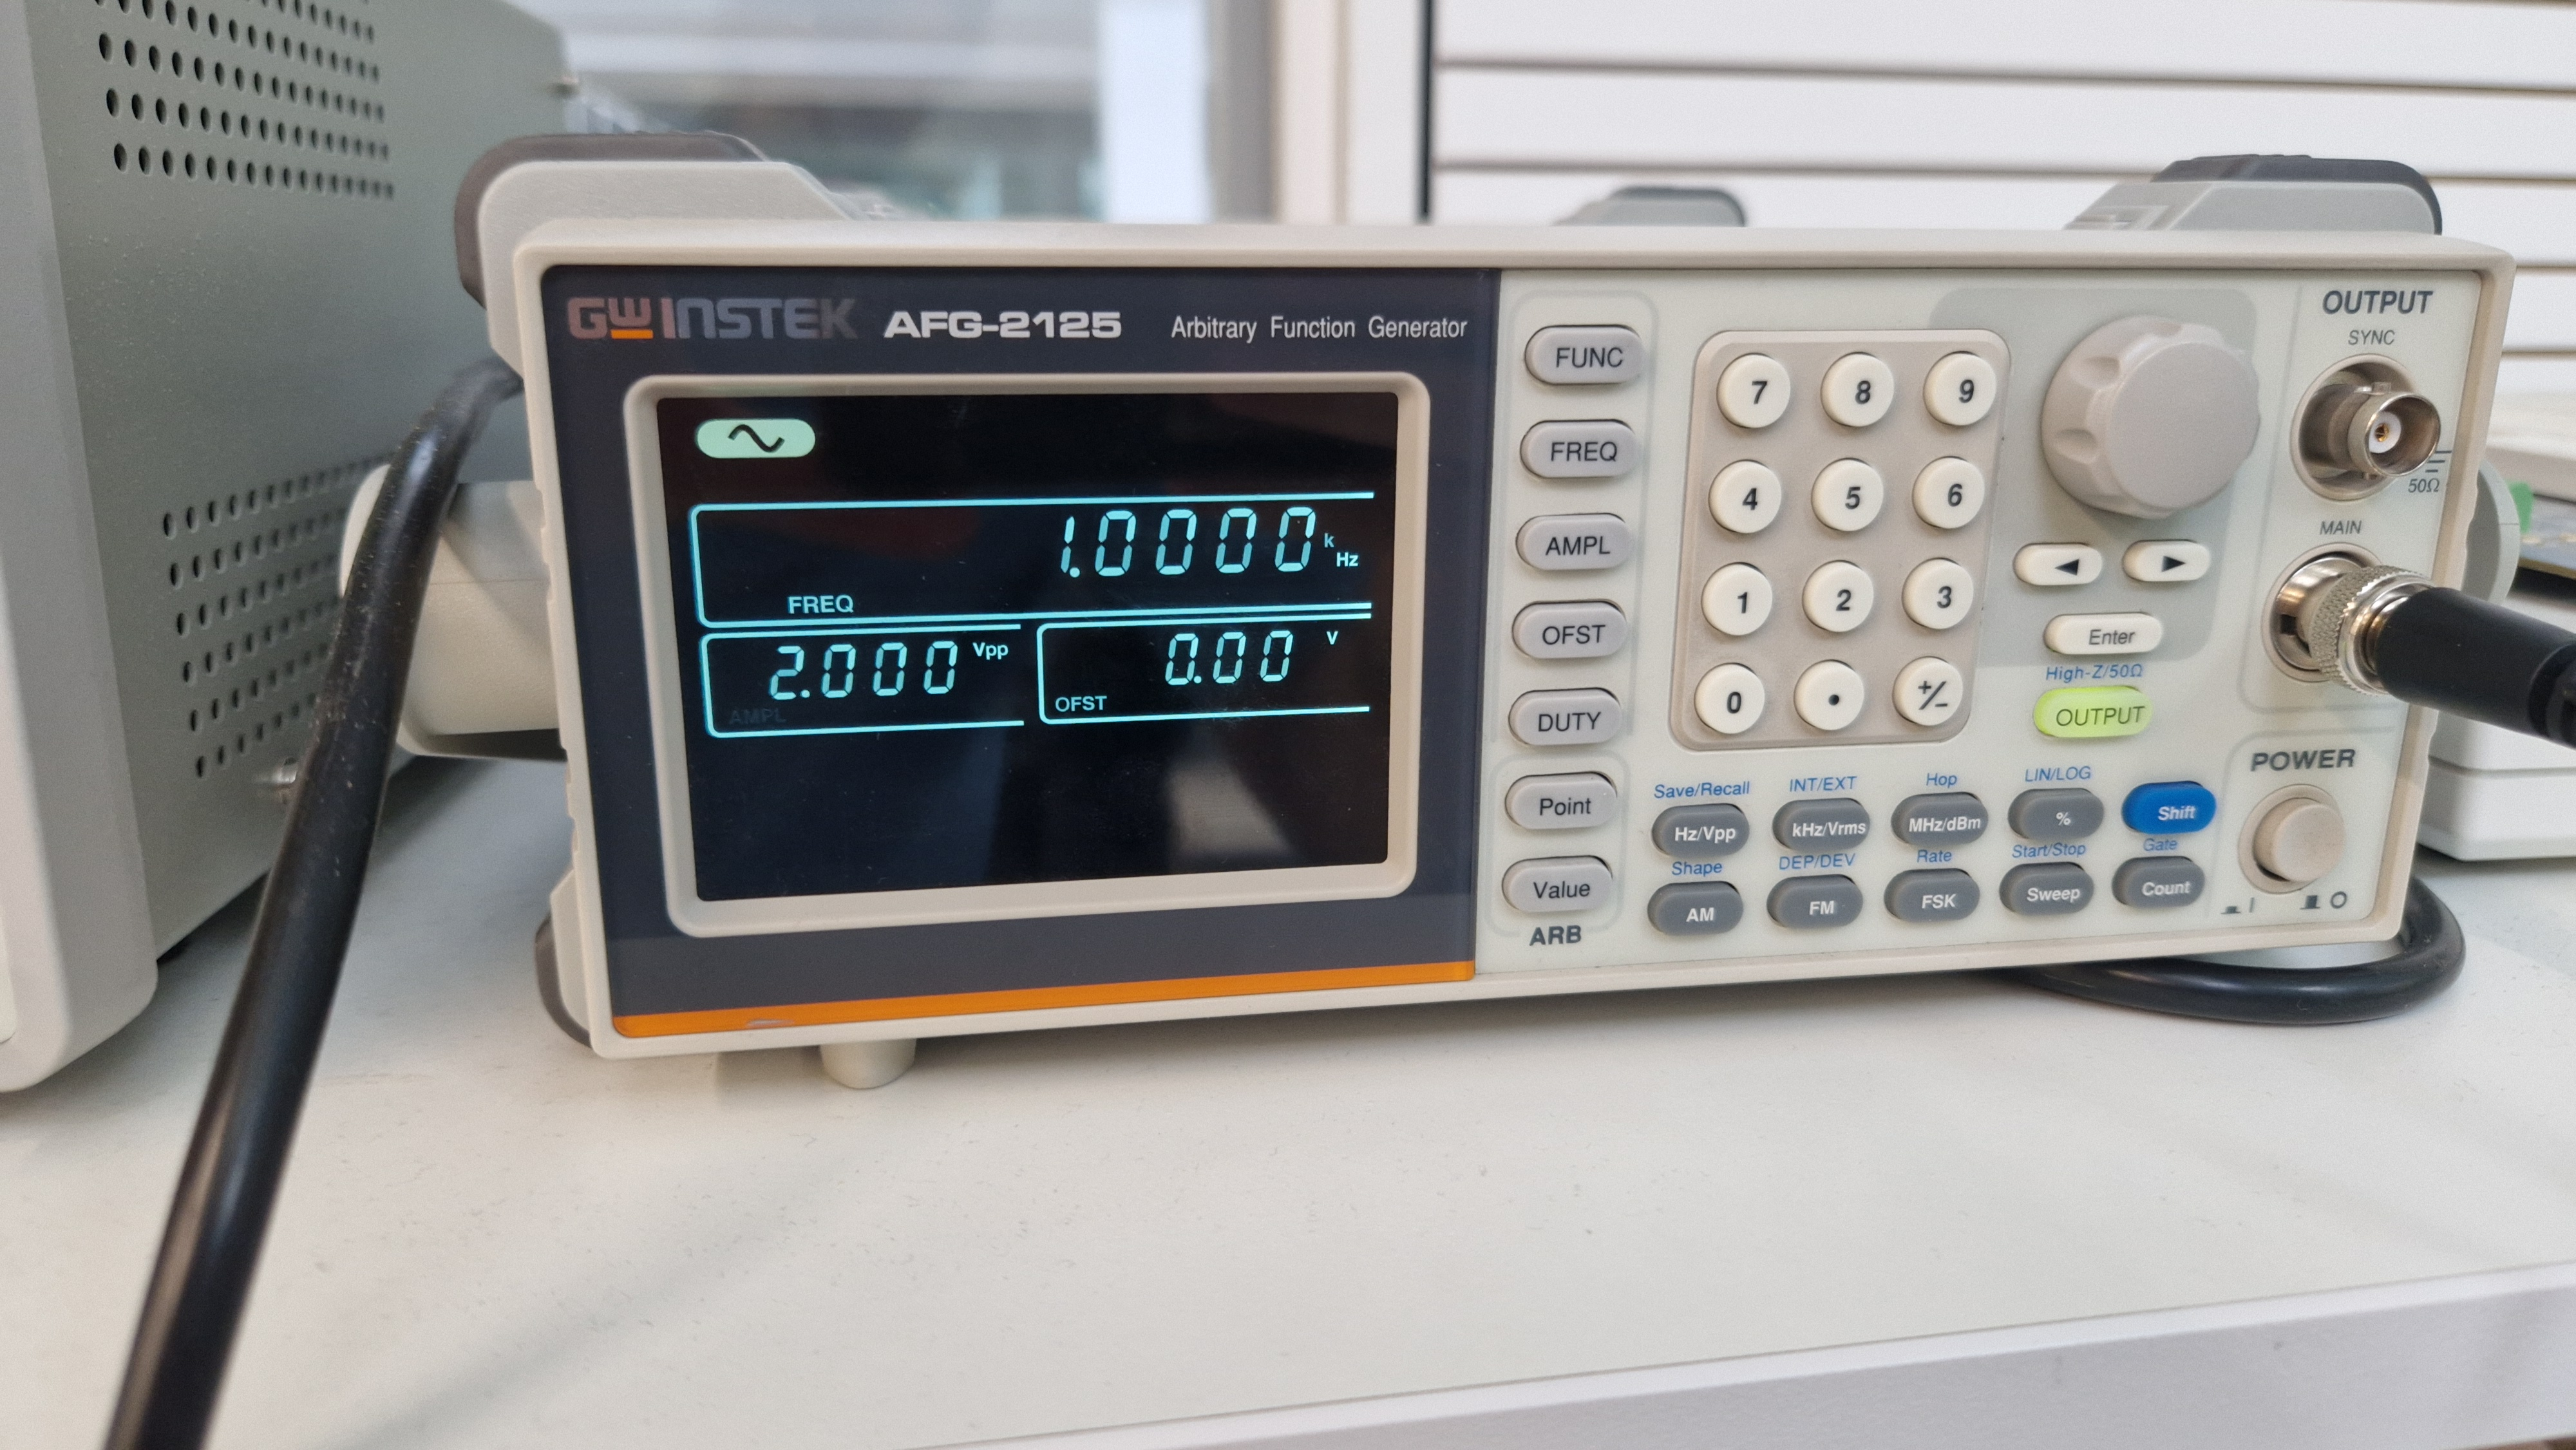
\includegraphics[width=0.6\textwidth]{assets/non-inverting-2.jpg}
    \caption{Signal Generator @ 2V}
    \label{fig:non-inverting-2}
\end{figure}

\begin{figure}[h]
    \centering
    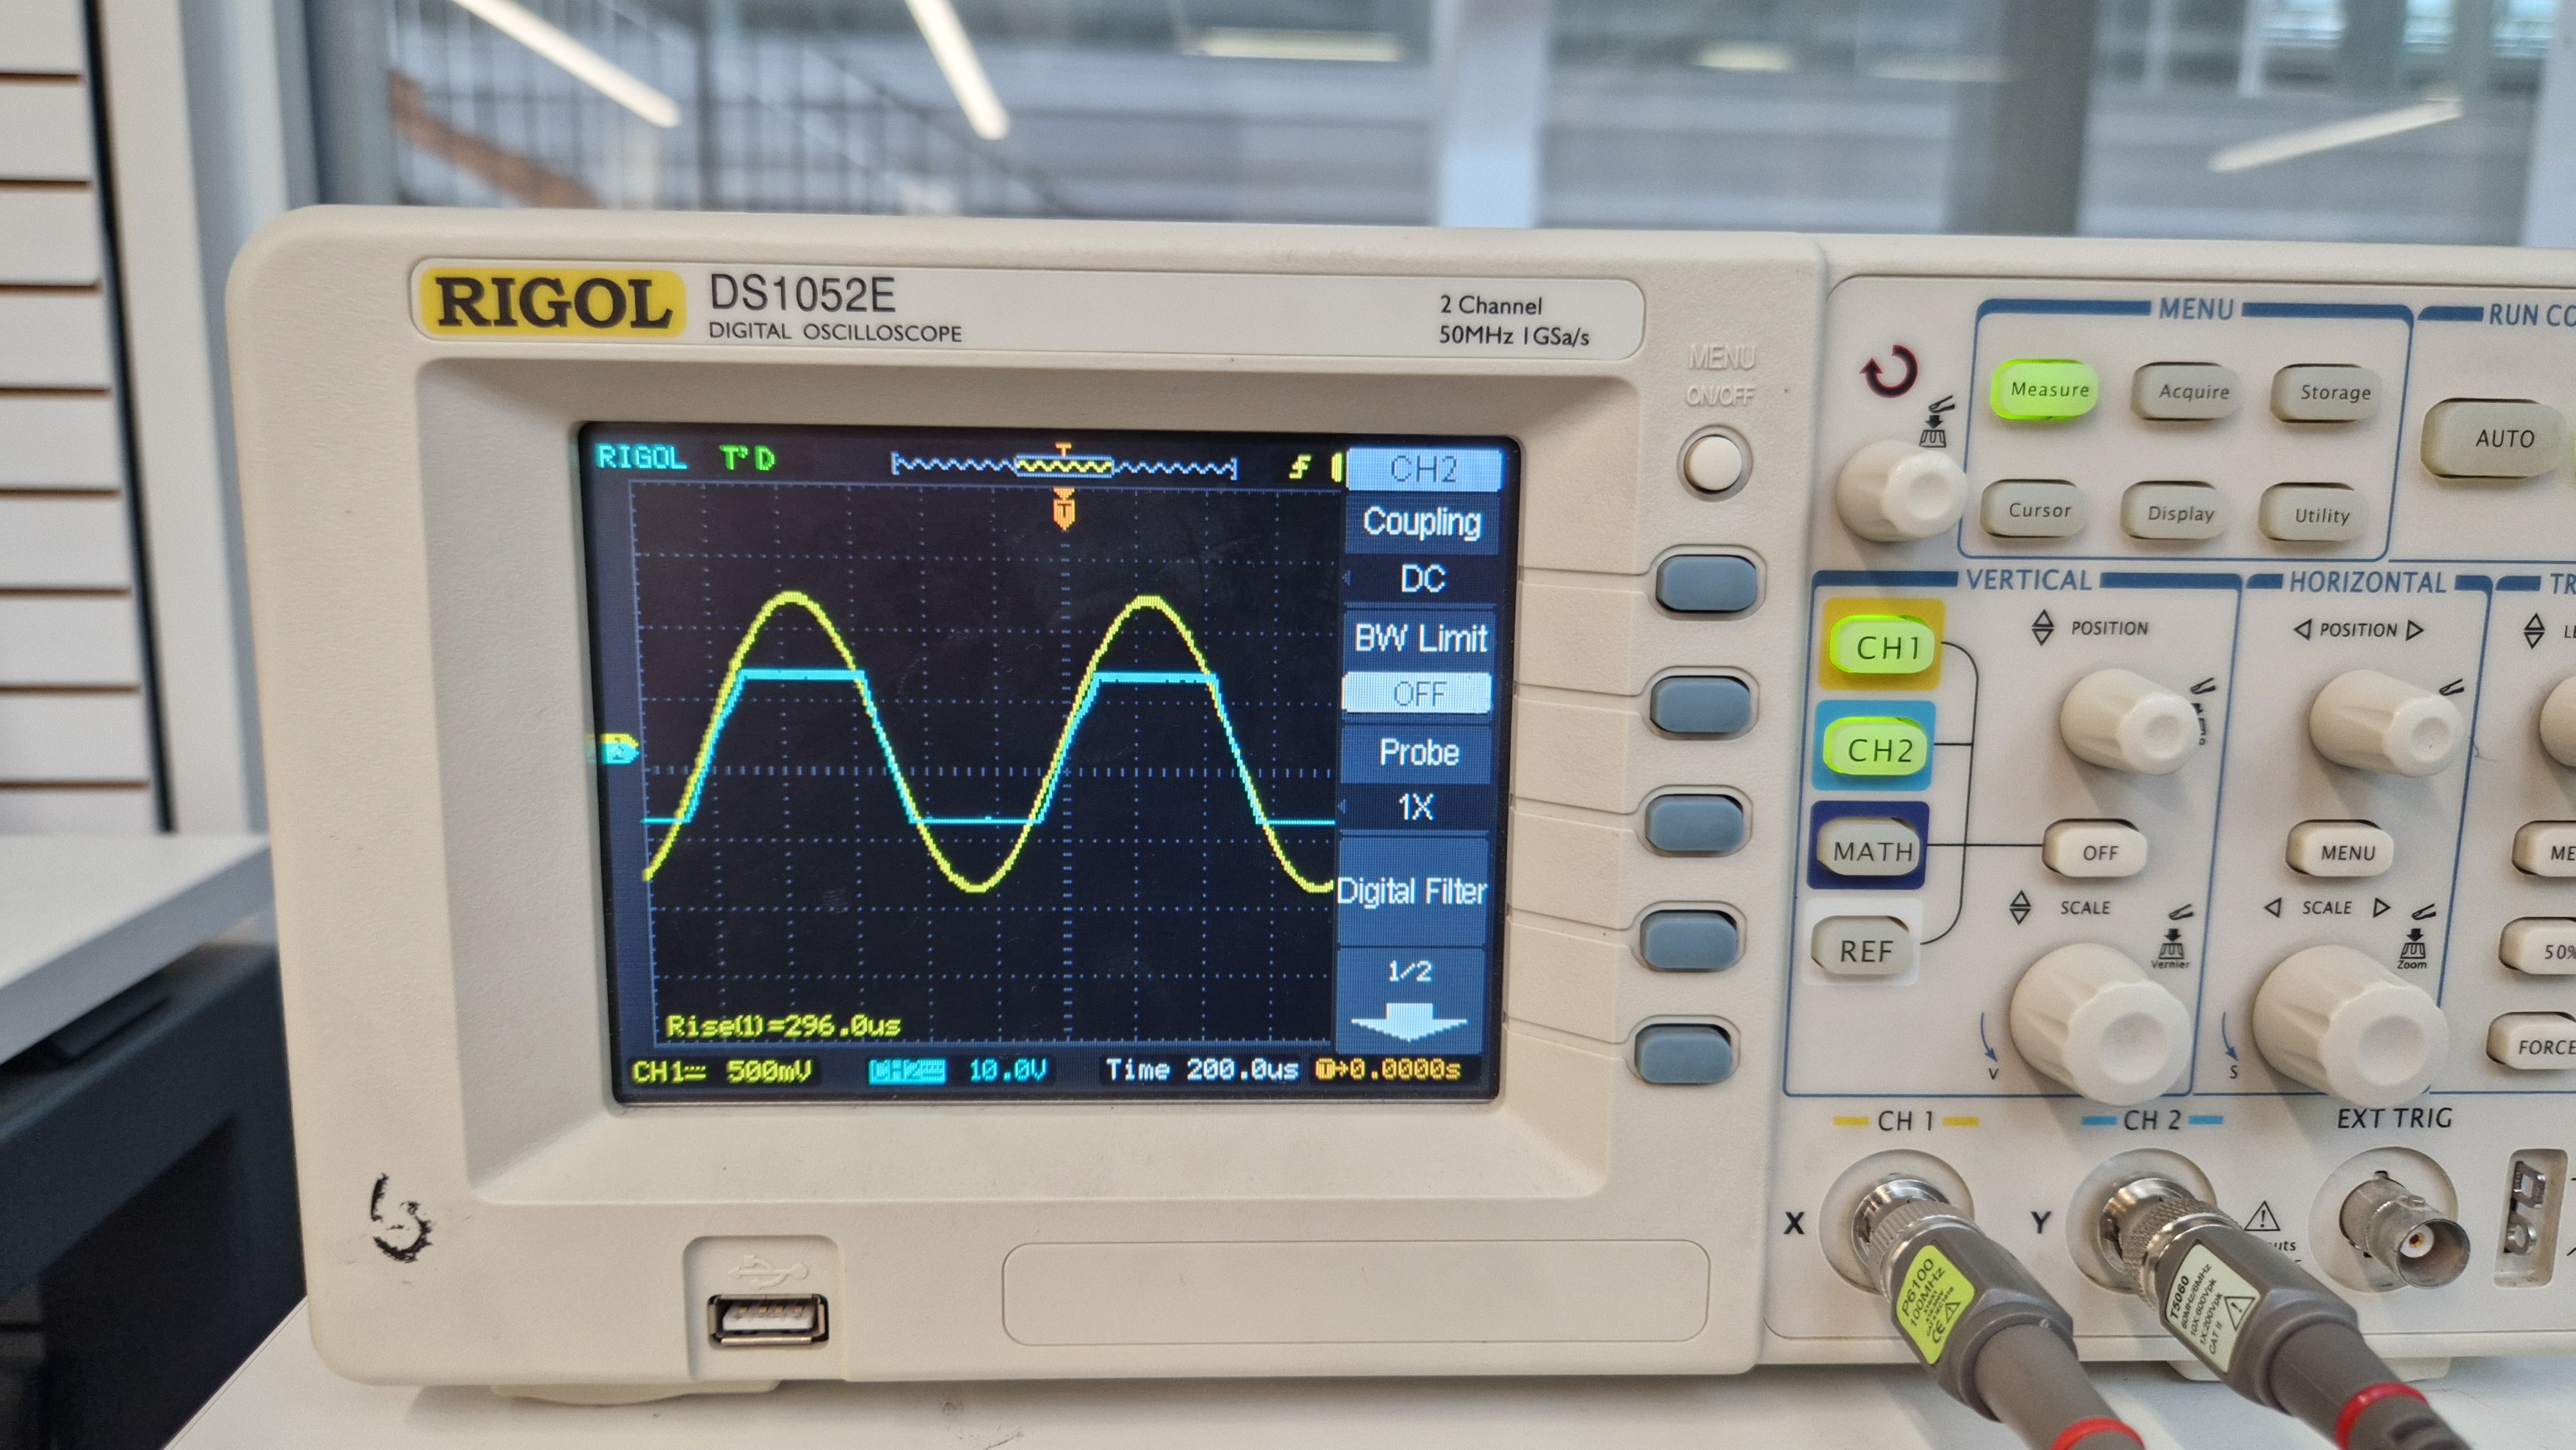
\includegraphics[width=0.6\textwidth]{assets/non-inverting-2-output.jpg}
    \caption{Non-inverting @ 2V}
    \label{fig:non-inverting-2-output}
\end{figure}

Applying 1V input to the non-inverting amplifier, the output should be 23V but it is limited to 12V due to the power supply as it is \textbf{more visible} in Figure \ref{fig:non-inverting-2-output}.

\newpage
\thispagestyle{plain}

\subsection{Inverting Amplifier}

\begin{figure}[h]
    \centering
    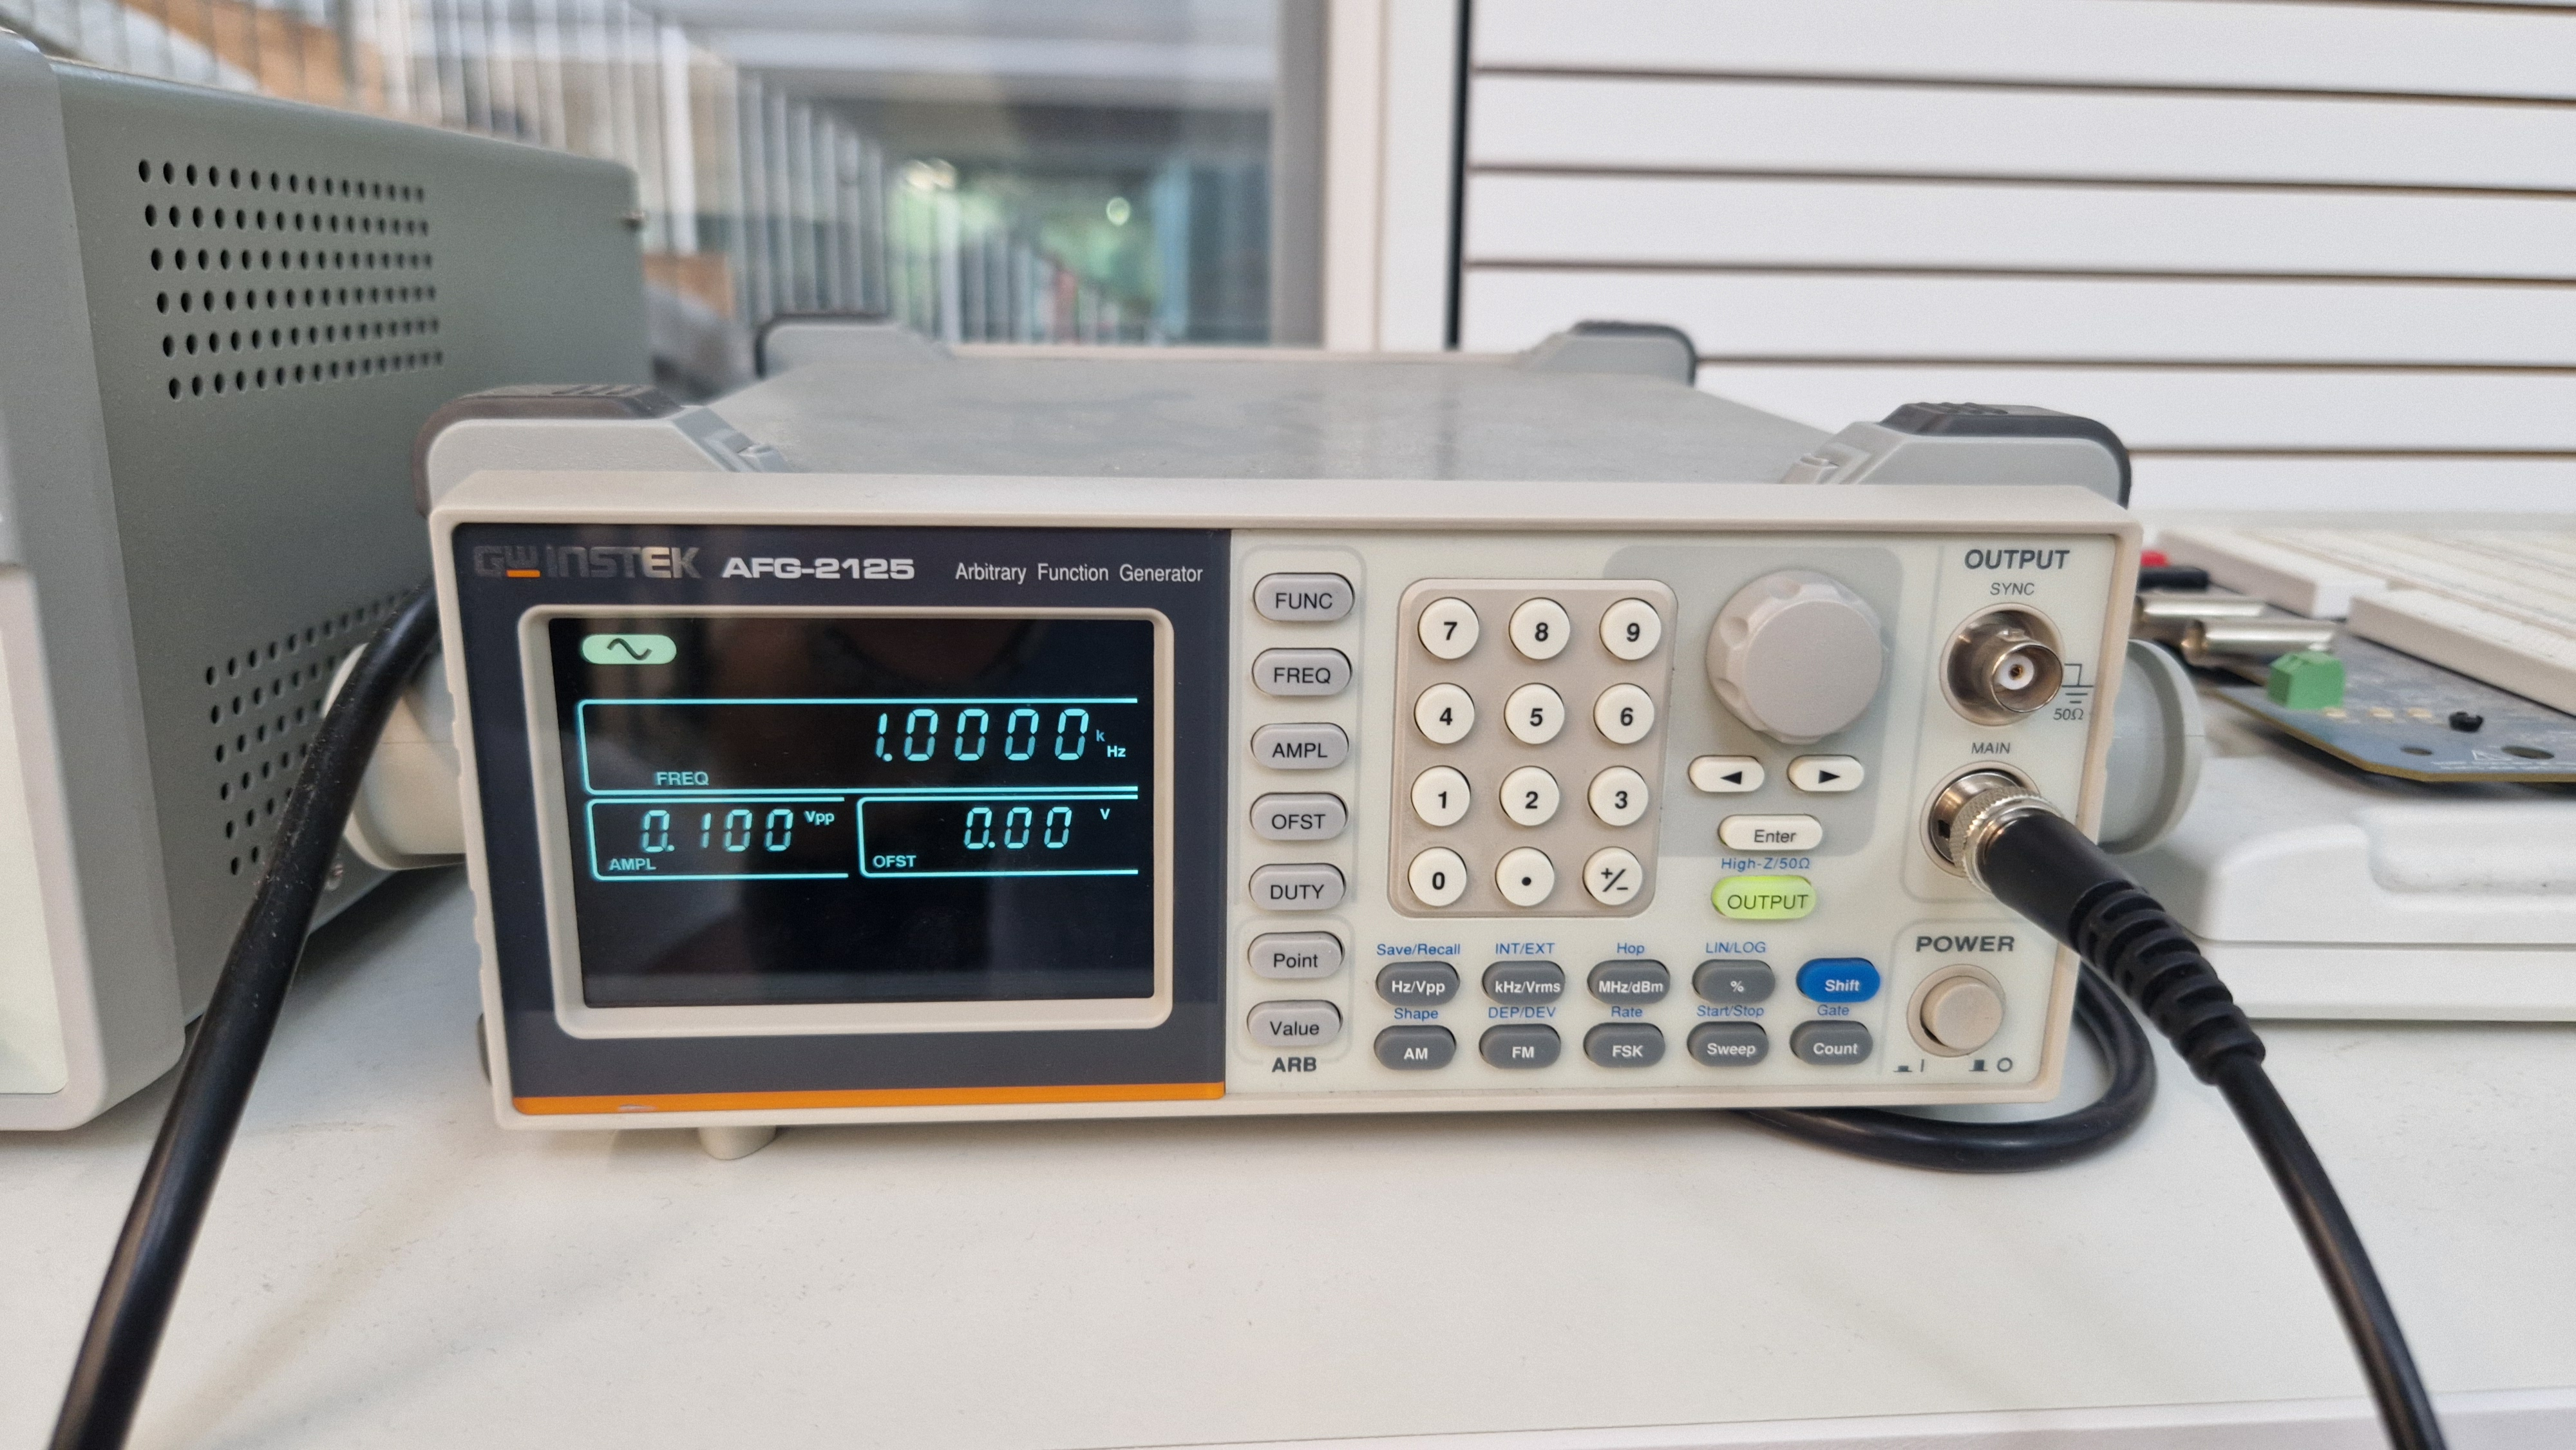
\includegraphics[width=0.6\textwidth]{assets/inverting-100.jpg}
    \caption{Signal Generator @ 100mV}
    \label{fig:inverting-100m}
\end{figure}

\begin{figure}[h]
    \centering
    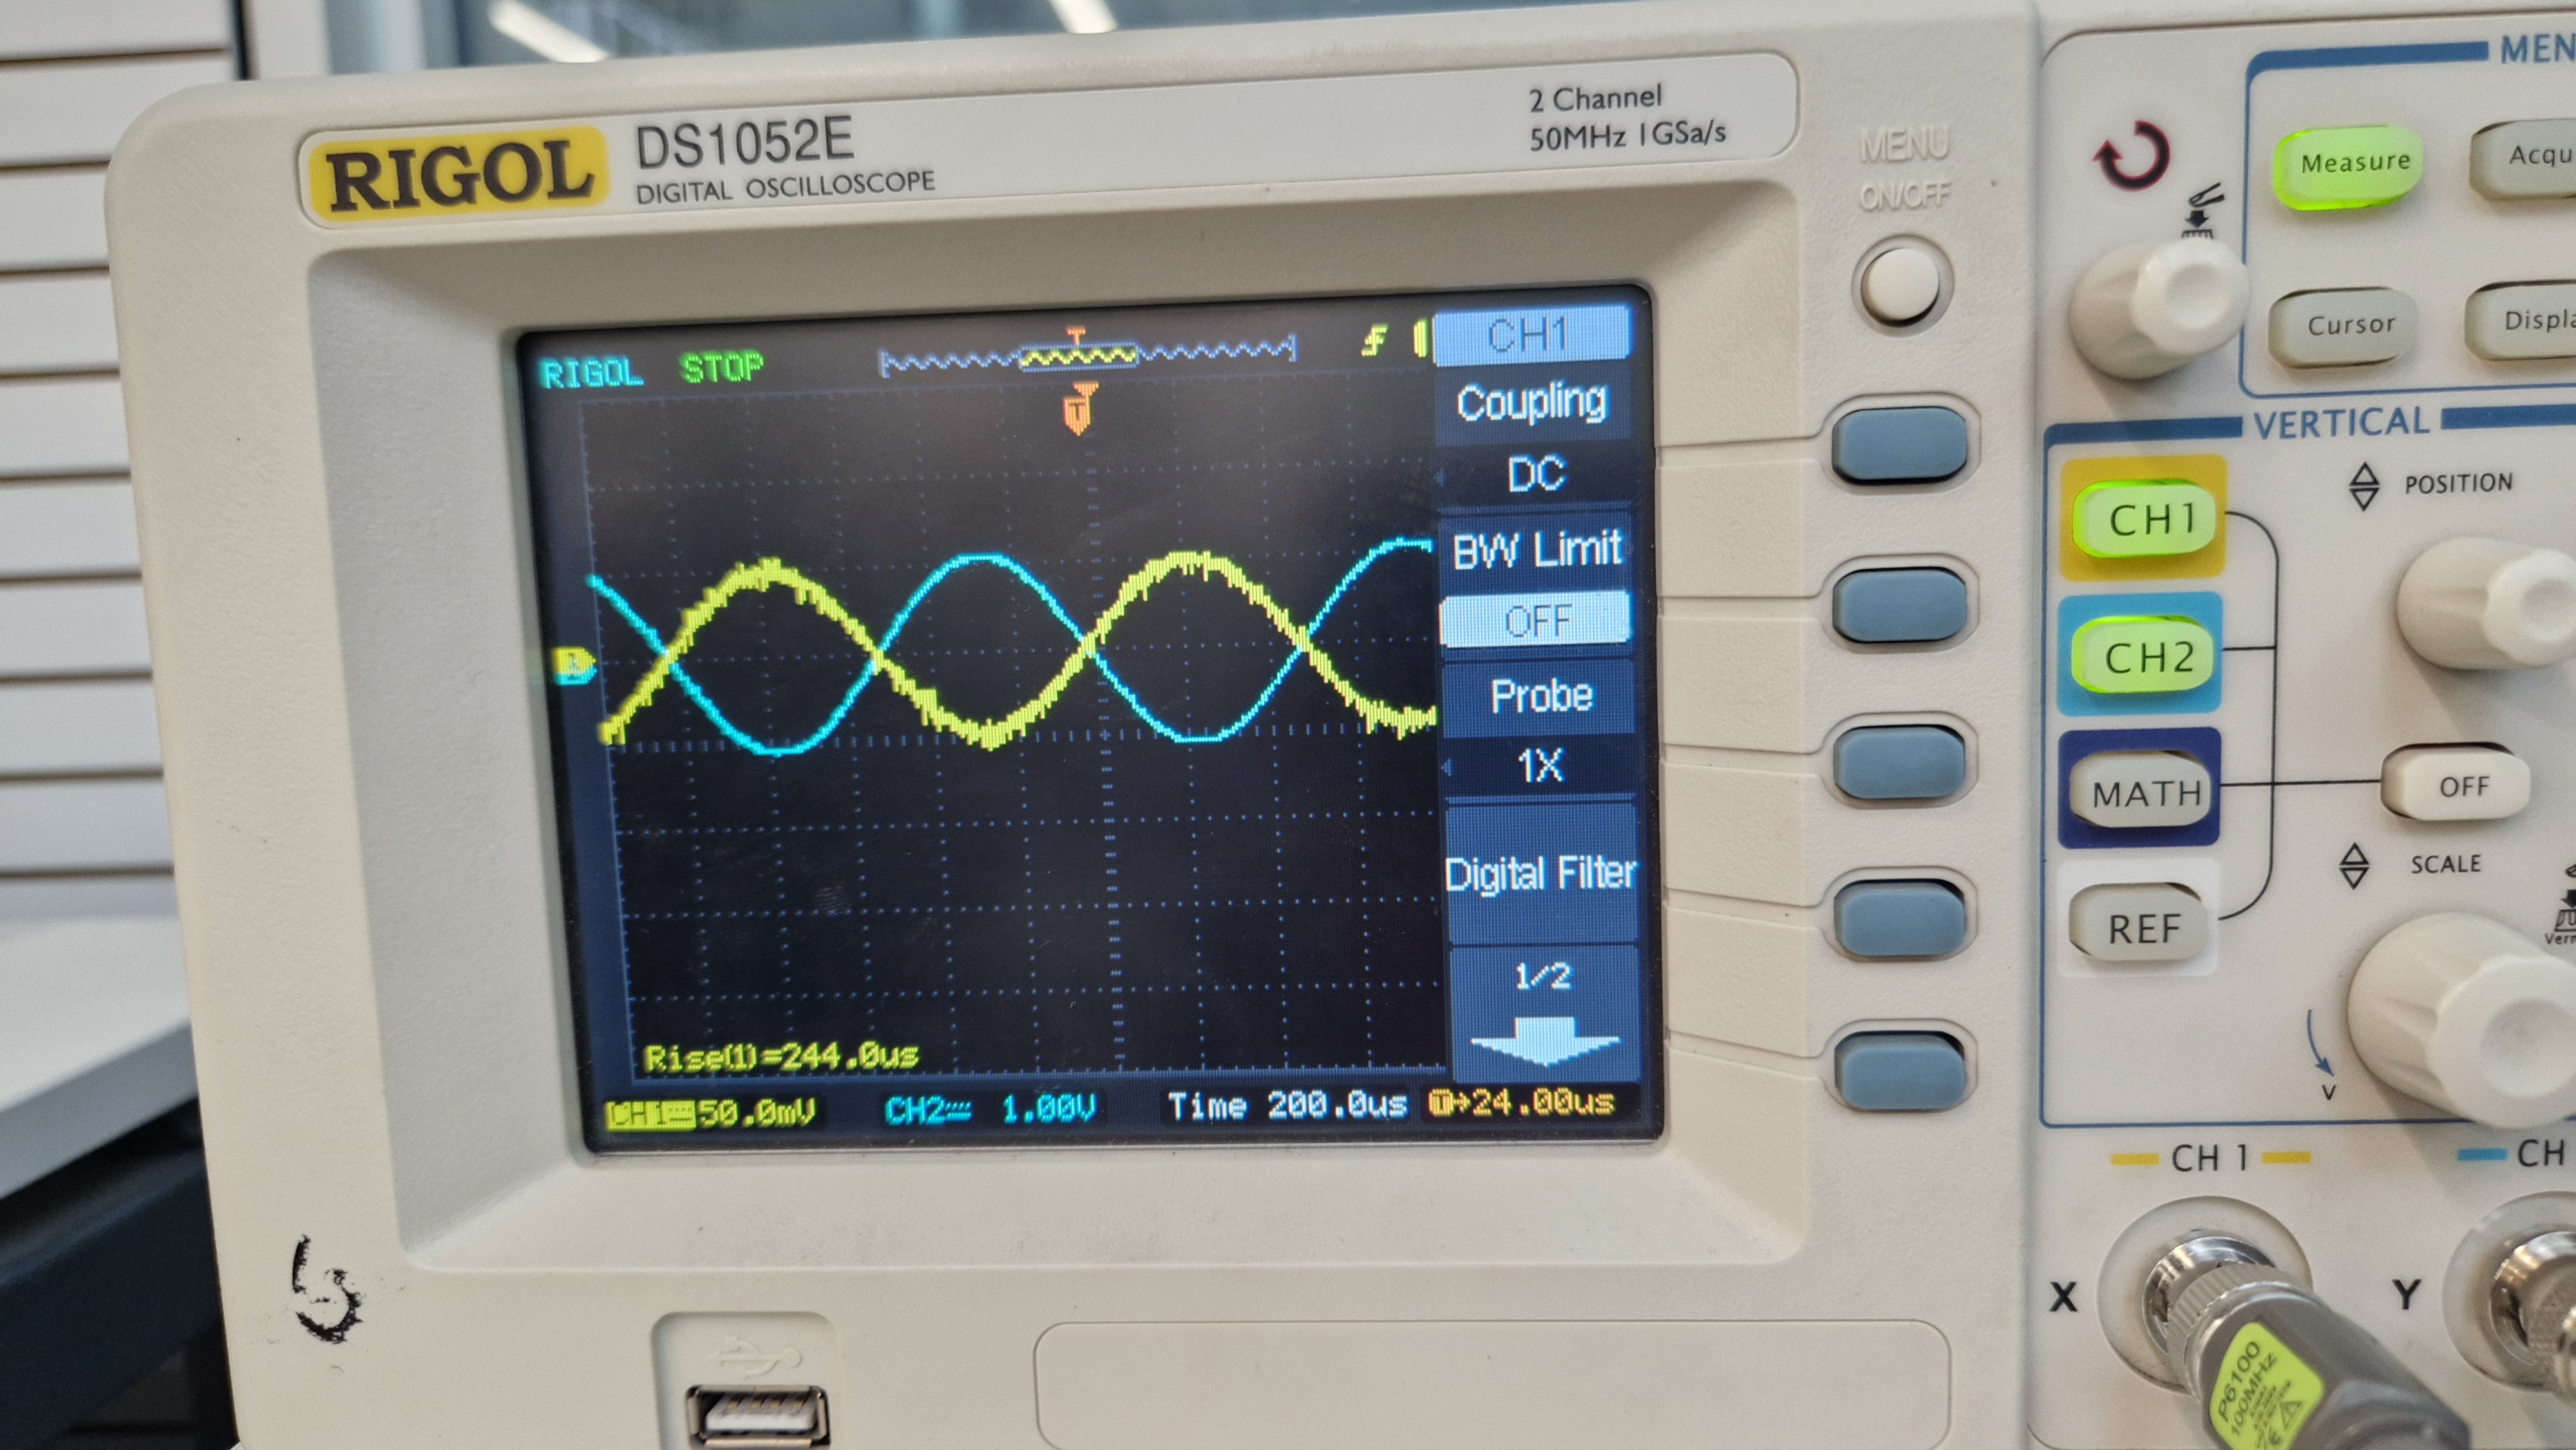
\includegraphics[width=0.6\textwidth]{assets/inverting-100-output.jpg}
    \caption{Inverting @ 100mV}
    \label{fig:inverting-100m-output}
\end{figure}

Applying 100mV input to the inverting amplifier, the output is close to -2.2V as expected. The experiment result is shown in Figure \ref{fig:inverting-100m-output}.

\newpage
\thispagestyle{plain}

\begin{figure}[h]
    \centering
    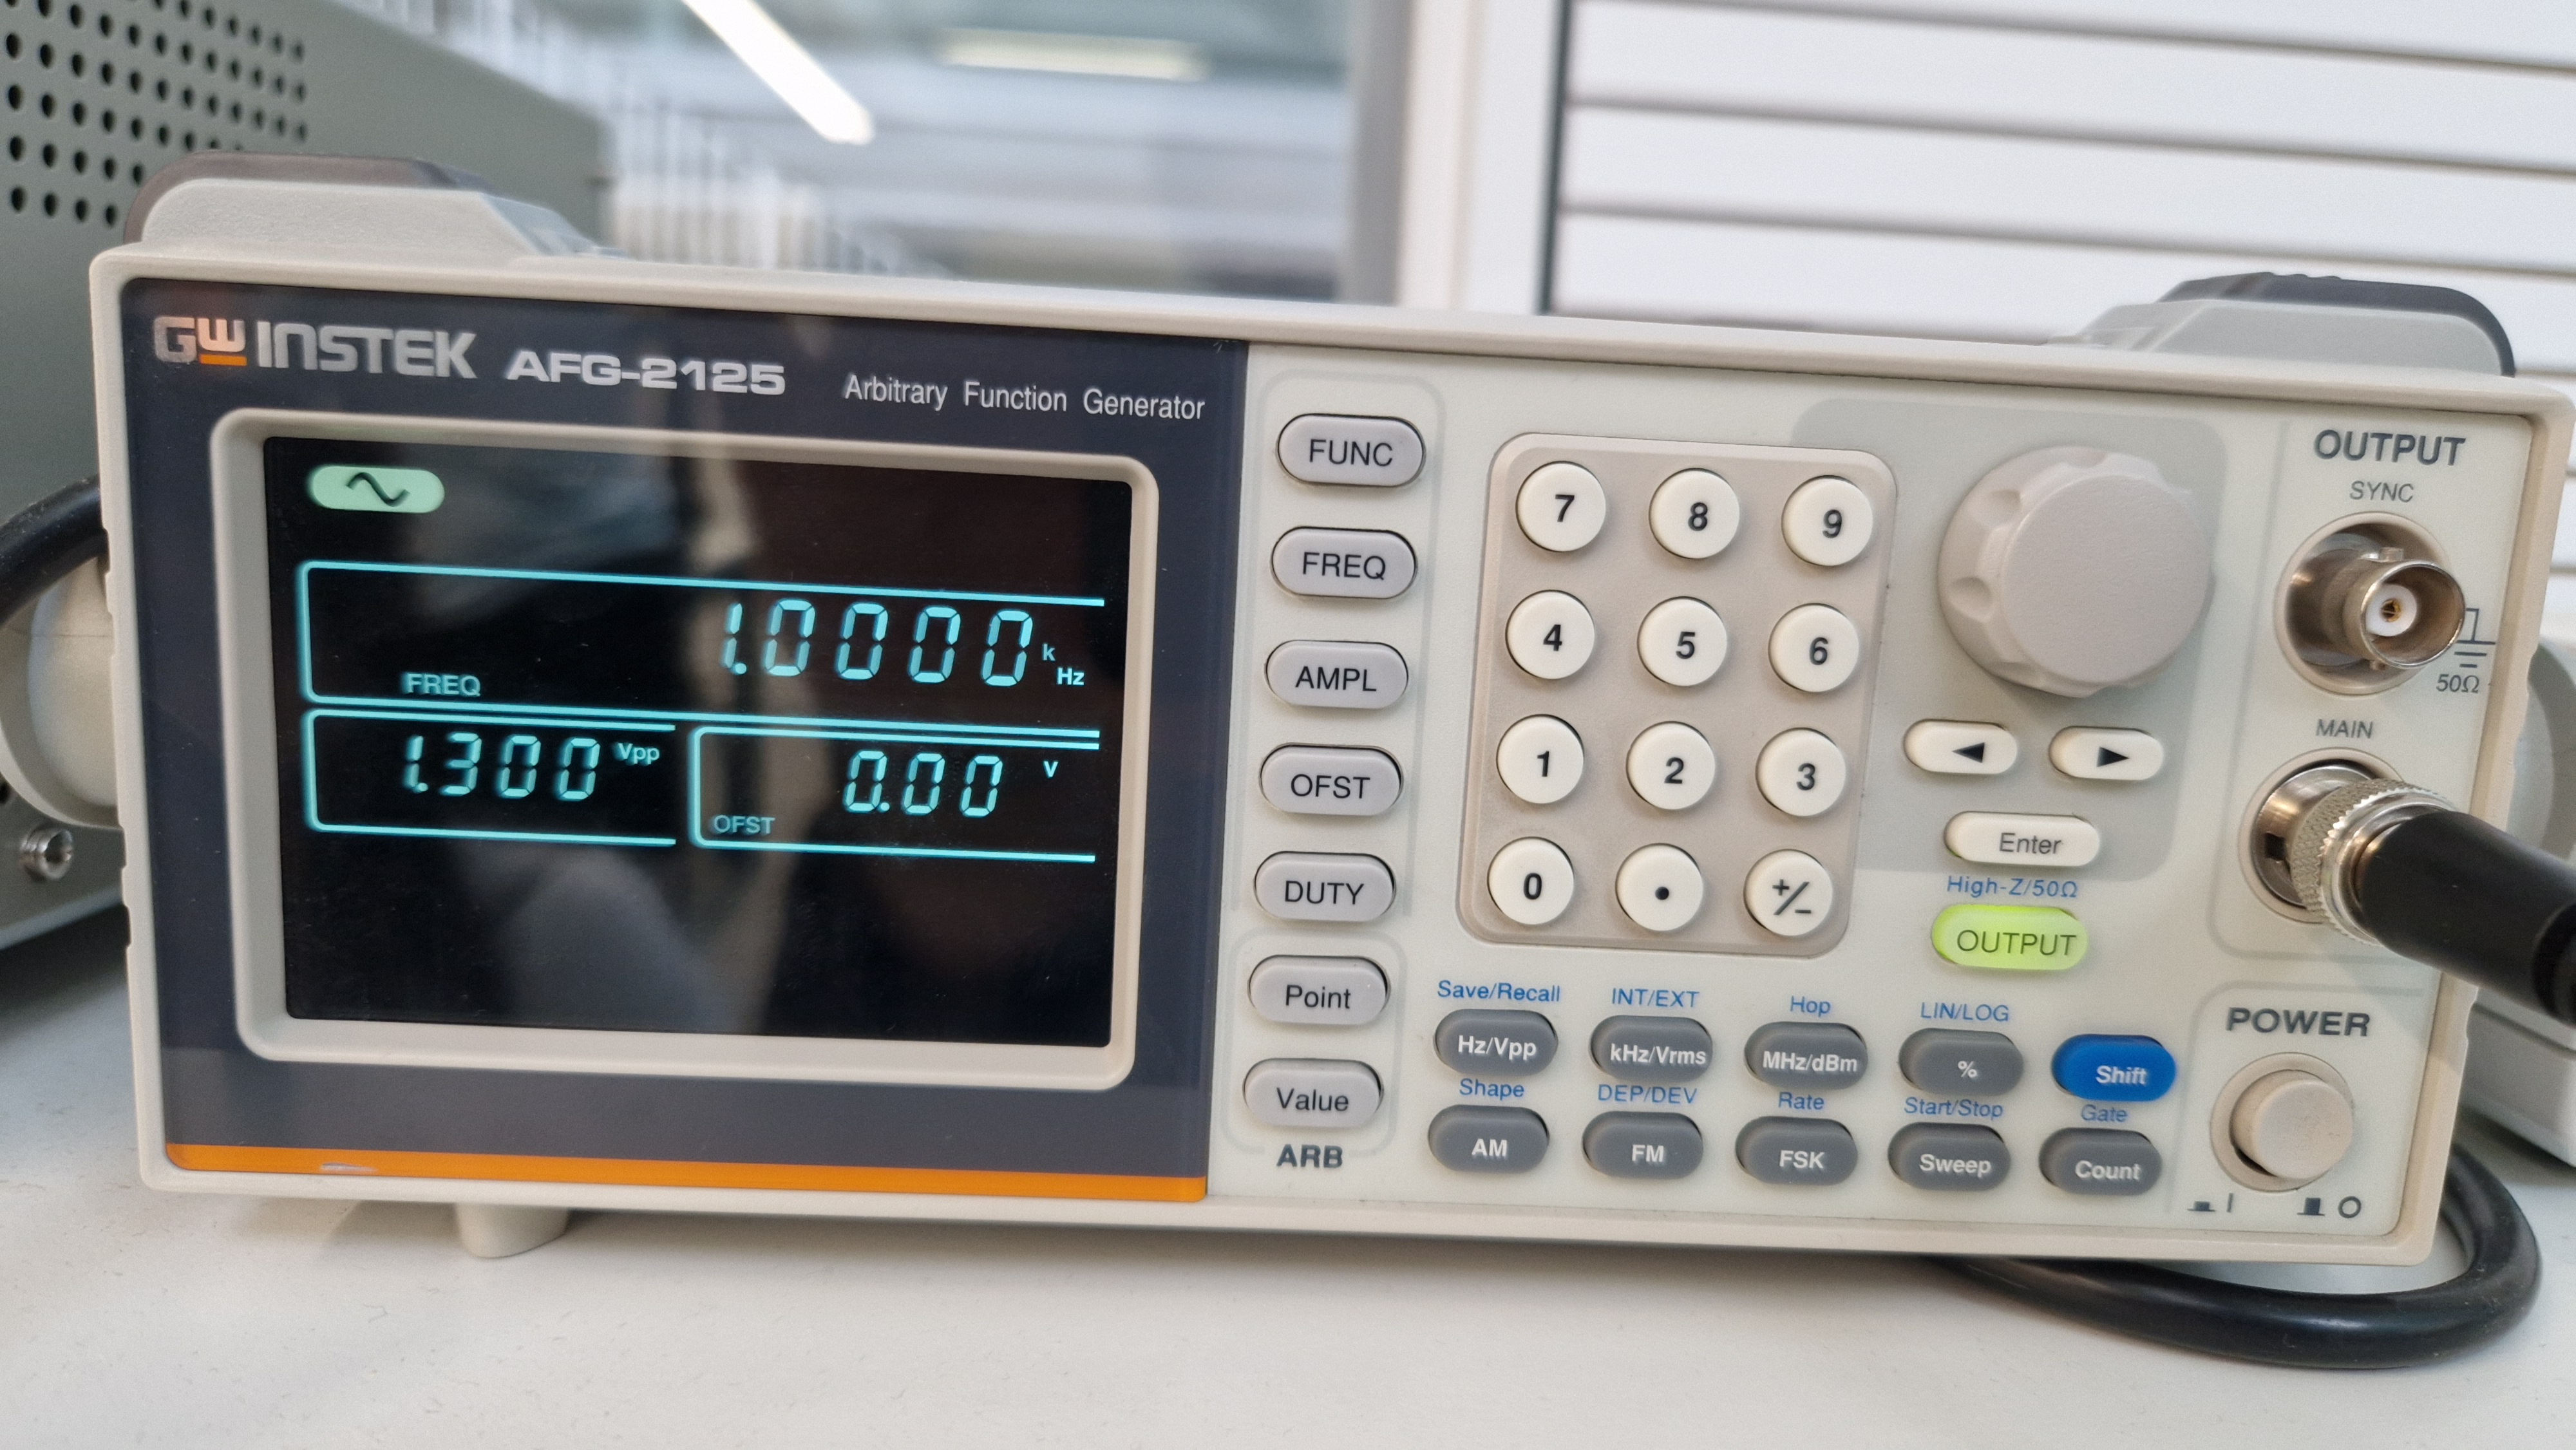
\includegraphics[width=0.6\textwidth]{assets/inverting-1.3.jpg}
    \caption{Signal Generator @ 1.3V}
    \label{fig:inverting-1.3}
\end{figure}

\begin{figure}[h]
    \centering
    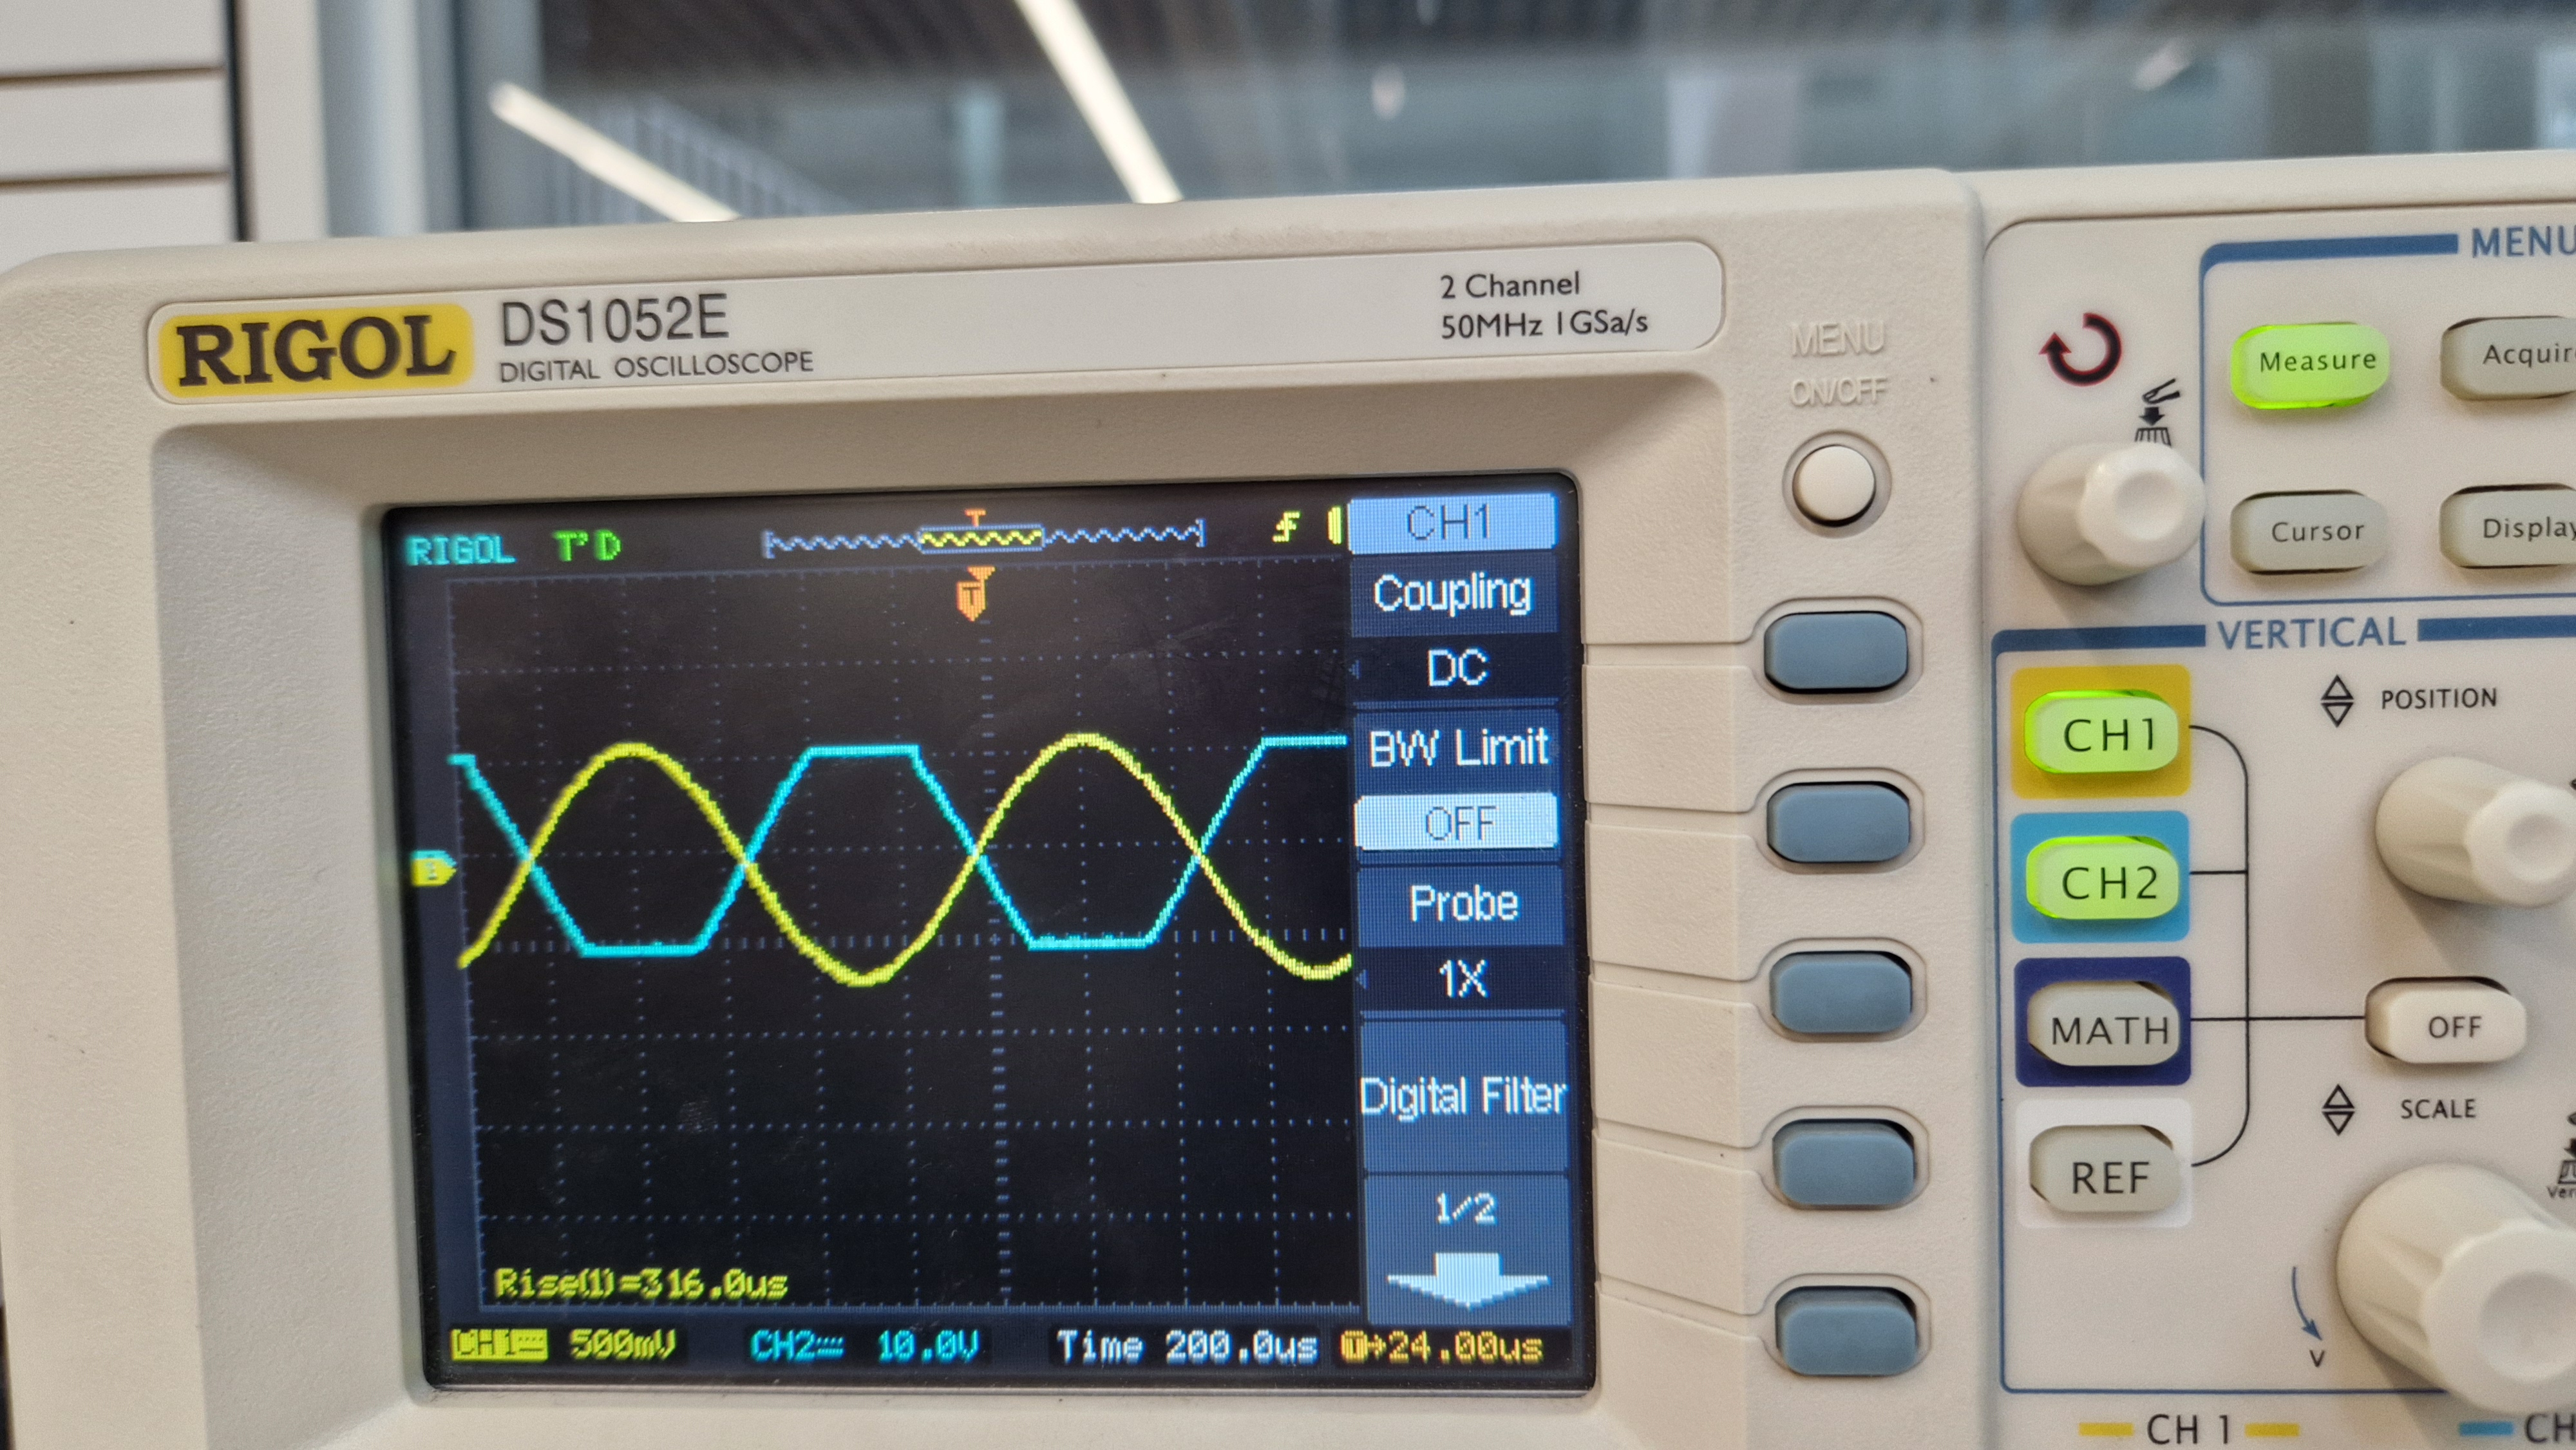
\includegraphics[width=0.6\textwidth]{assets/inverting-1.3-output.jpg}
    \caption{Inverting @ 1.3V}
    \label{fig:inverting-1.3-output}
\end{figure}

Applying 1.3V input to the inverting amplifier, the output should be -28.6V but it is limited to -12V due to the power supply as seen in Figure \ref{fig:inverting-1.3-output}.

\newpage
\thispagestyle{plain}

\begin{figure}[h]
    \centering
    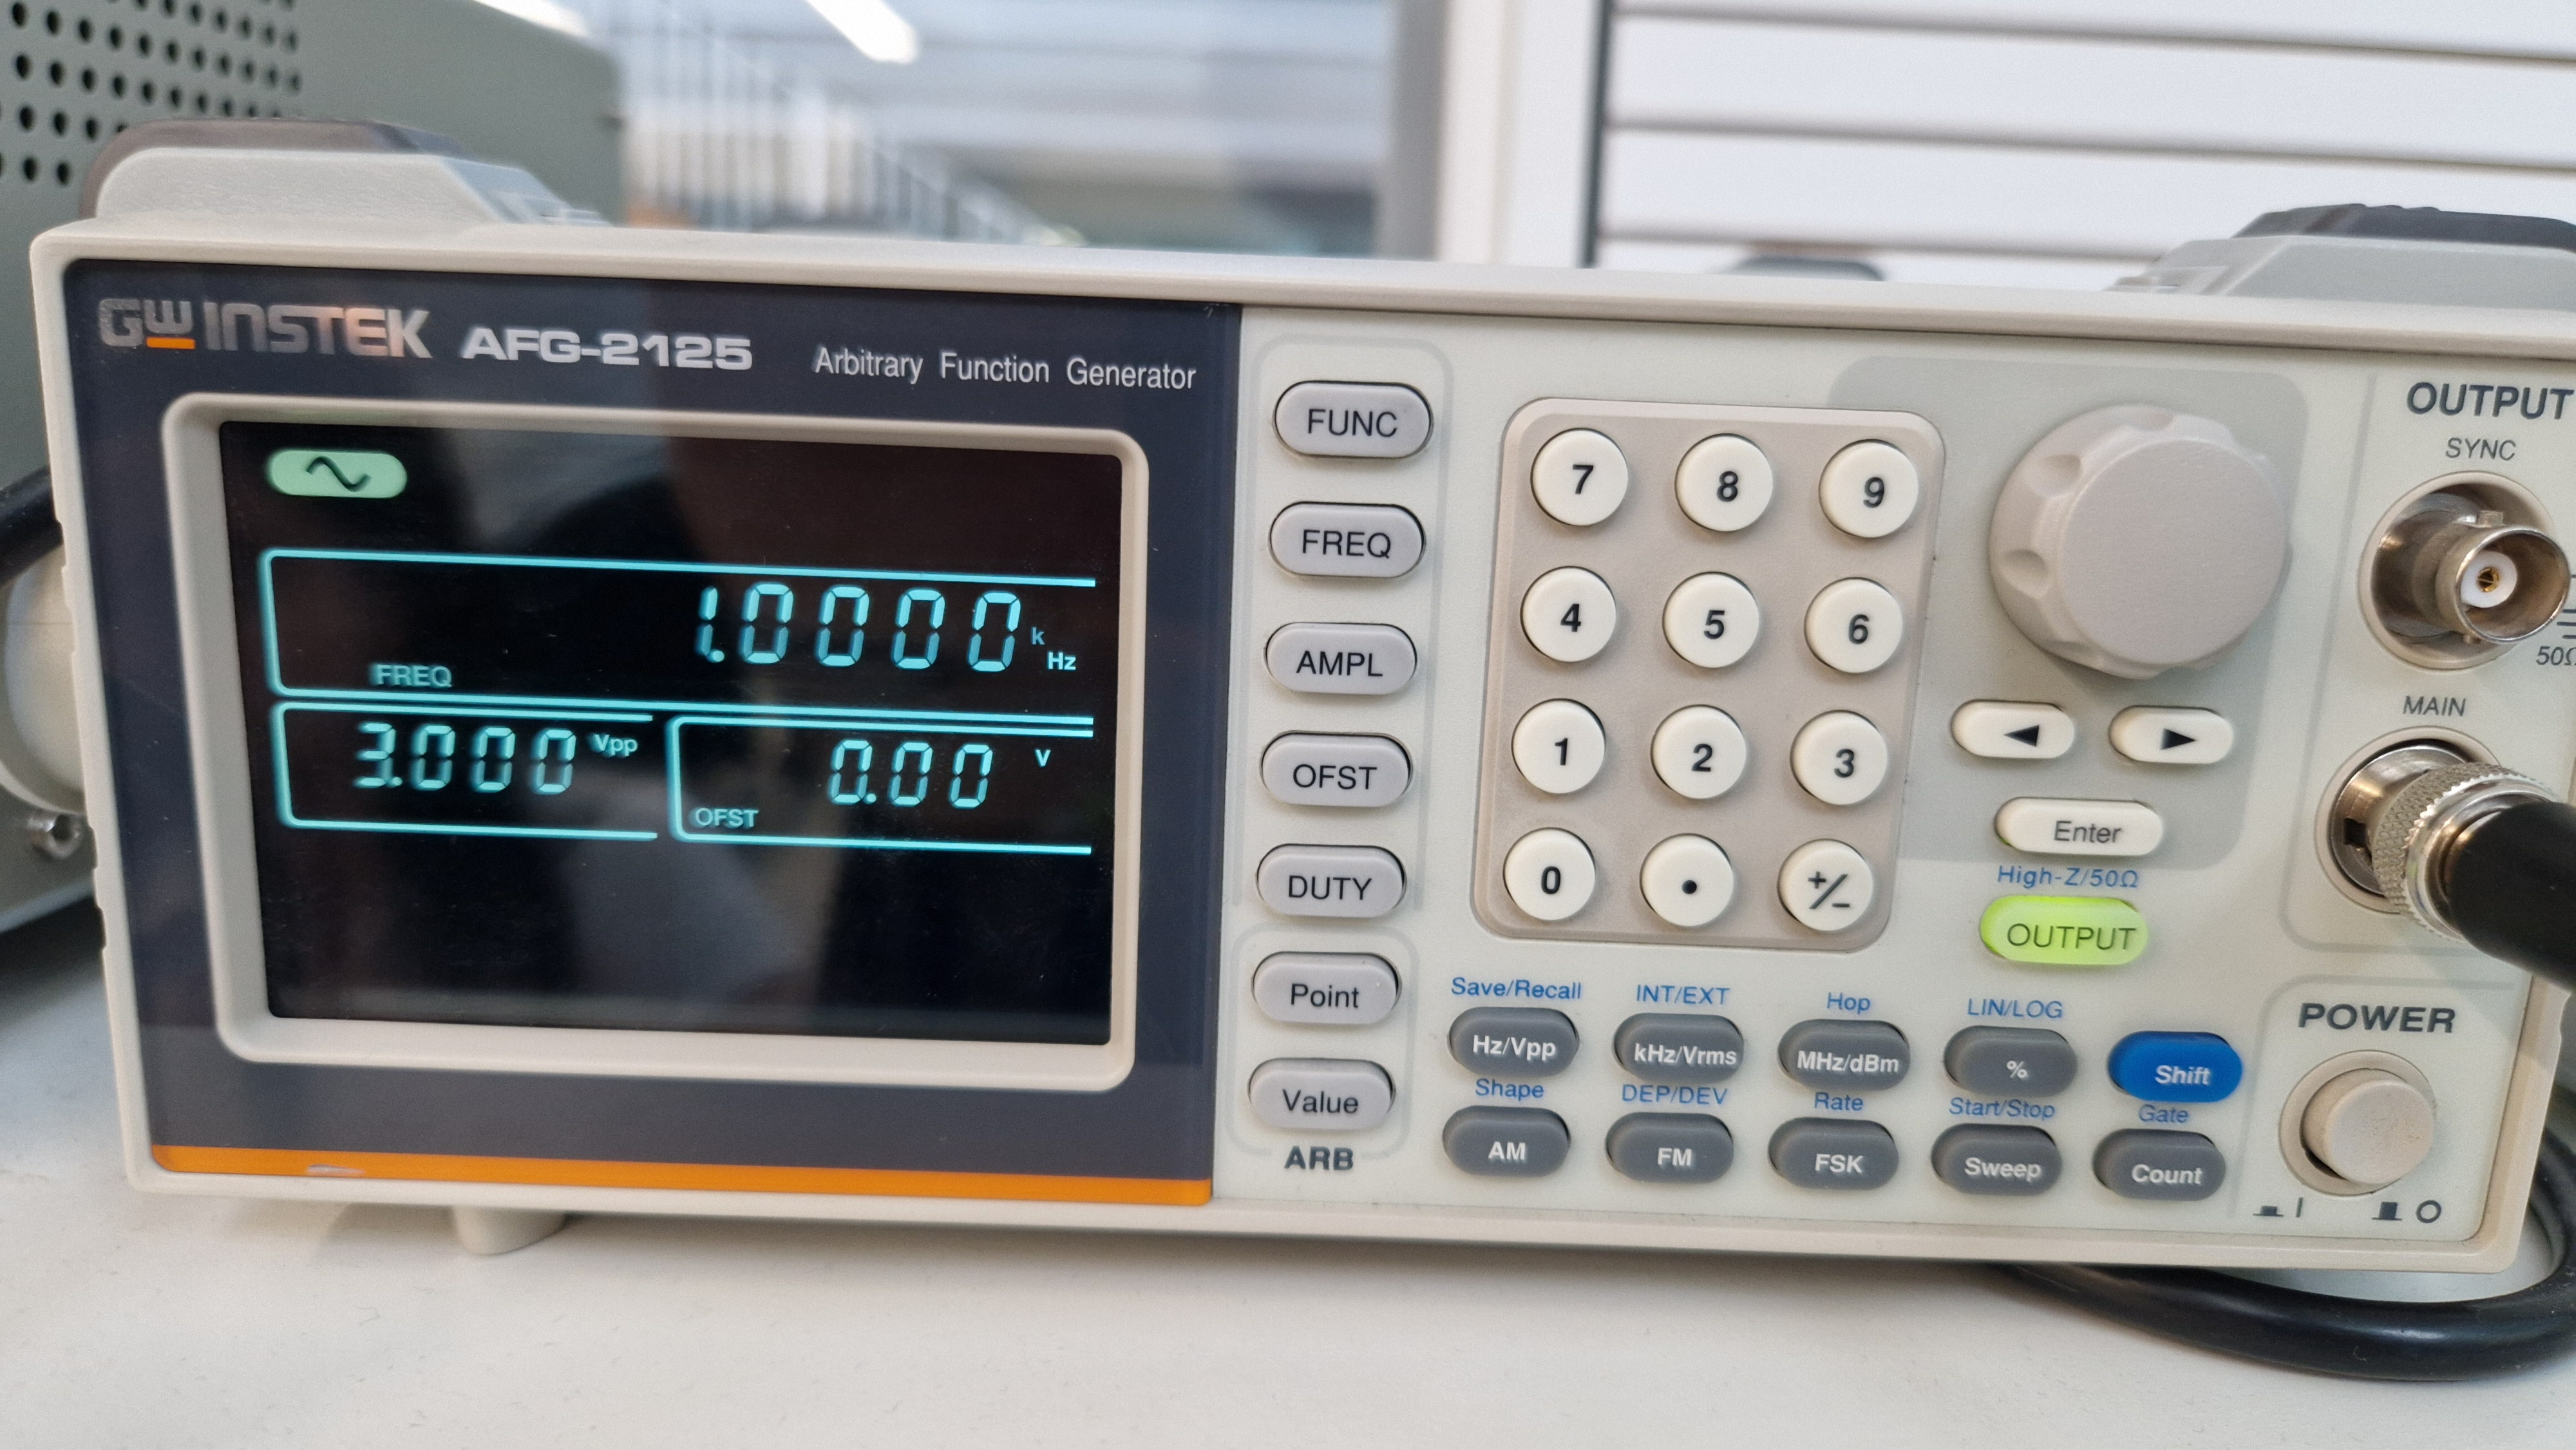
\includegraphics[width=0.6\textwidth]{assets/inverting-3.jpg}
    \caption{Signal Generator @ 3V}
    \label{fig:inverting-3}
\end{figure}

\begin{figure}[h]
    \centering
    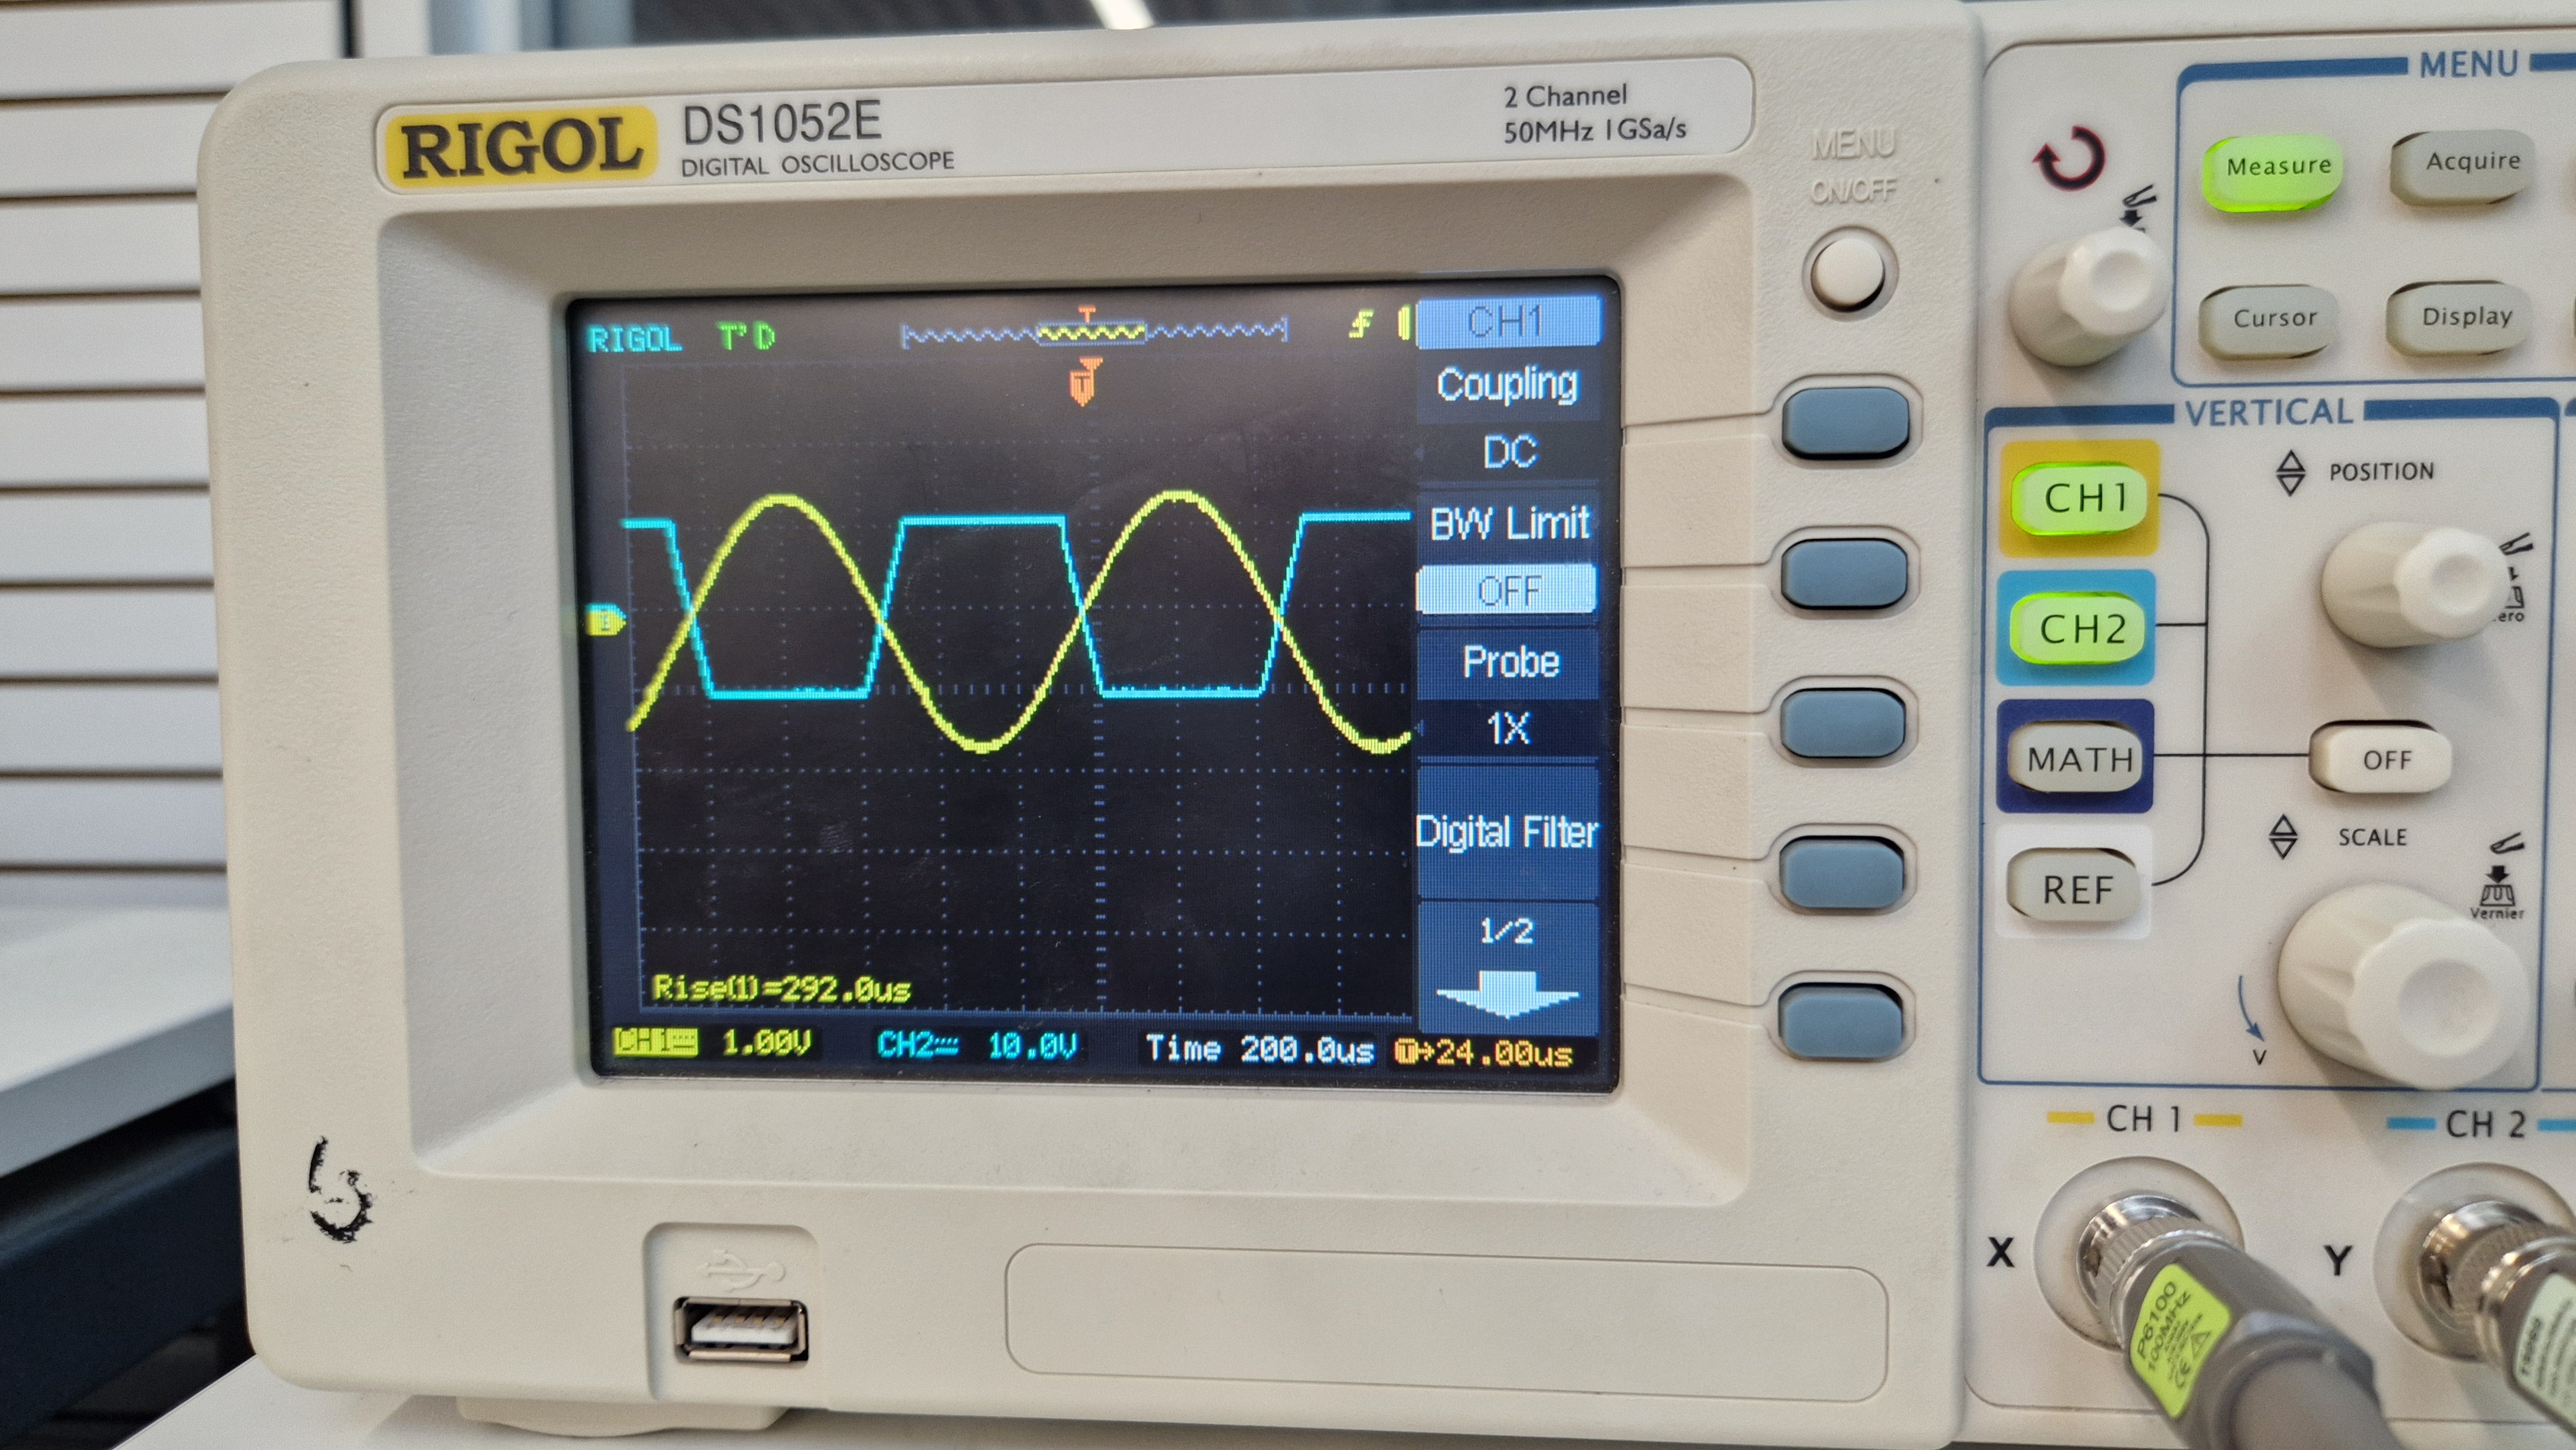
\includegraphics[width=0.6\textwidth]{assets/inverting-3-output.jpg}
    \caption{Inverting @ 3V}
    \label{fig:inverting-3-output}
\end{figure}

Applying 3V input to the inverting amplifier, the output should be -66V but it is limited to -12V due to the power supply as it is \textbf{more visible} in Figure \ref{fig:inverting-3-output}.
